\documentclass[11pt,a4paper]{article}
\usepackage[margin=24mm]{geometry}
\usepackage[T1]{fontenc}
\usepackage{lmodern,microtype,booktabs,tabularx,array,graphicx,xcolor,amsmath}
\usepackage[most]{tcolorbox}
\usepackage{tikz}
\usetikzlibrary{positioning,arrows.meta}
\usepackage[numbers,sort&compress]{natbib}
\usepackage[hypertexnames=false,colorlinks=true,linkcolor=blue!45!black,urlcolor=blue!45!black,citecolor=blue!45!black]{hyperref}
\usepackage{fancyhdr}
\pagestyle{fancy}\fancyhf{}\fancyfoot[C]{\thepage}\renewcommand{\headrulewidth}{0pt}
\setlength{\headheight}{14pt}
\setlength{\emergencystretch}{2em}
\setlength{\parindent}{0pt}\setlength{\parskip}{6pt}
\newcolumntype{Y}{>{\raggedright\arraybackslash}X}
\newcommand{\todo}[1]{\begingroup\setlength{\fboxsep}{2pt}\colorbox{yellow!45}{\strut\textbf{TODO:} #1}\endgroup}
\newtcolorbox{review}[1]{colback=yellow!12,colframe=orange!65!black,title={REVIEW: #1},fonttitle=\bfseries,boxrule=0.6pt}
\newcommand{\aistars}[1]{\foreach \n in {1,...,5}{\ifnum\n>#1\relax\textcolor{gray!40}{$\star$}\else\textcolor{orange!80!black}{$\star$}\fi}}
% Temporary internal review assignments: change to \draftreviewersfalse to hide.
\newif\ifdraftreviewers
\draftreviewerstrue
\newcommand{\draftreview}[3]{\ifdraftreviewers\textbf{Draft reviewers: #1 (lead); #2 (support).} #3\par\smallskip\fi}
\newcommand{\pending}{\textcolor{orange!70!black}{\textbf{Pending}}}
\newcommand{\assetplaceholder}[2]{\begin{review}{#1}\centering\vspace{8mm}\par\textit{#2}\par\vspace{8mm}\end{review}}
\begin{document}
\raggedbottom
\begin{titlepage}
\centering
{\large Nanyang Technological University\par}
{\large AI6127: Deep Neural Networks for Natural Language Processing\par}
\vspace{17mm}
{\LARGE Evidence-grounded question answering over NLP research papers\par}
\vspace{9mm}
{\large Assignment report --- review draft\par}
{Due: 7 November 2026\par}\vspace{8mm}
Group number: 24\par\vspace{6mm}
\begin{tabularx}{\textwidth}{Yr}\toprule
Member name (alphabetical order) & Matriculation number\\\midrule
Ananya Redhu & \todo{matriculation number}\\
Changyan Xu & G2607680G\\
Jingshuai Qian & \todo{matriculation number}\\
Junlin Yin & \todo{matriculation number}\\
Junyu Hu & \todo{matriculation number}\\
Maheshwari Vishakha Praveen & \todo{matriculation number}\\\bottomrule
\end{tabularx}
\vspace{6mm}
\begin{review}{Submission metadata}
Members are listed alphabetically by displayed full name. Confirm official spellings and name order against university records. Names are taken from the project README and annotation audit; the audit also records Junyu Hu as ``HU JUNYU.'' Add the remaining matriculation numbers above. Select the Blackboard submitter.
\end{review}
\vfill
\begin{review}{Draft status}
Available measurements are development results, not final held-out scores. Yellow review boxes identify missing evidence, unresolved decisions and suggestions. Pending entries are not zero scores. Final QA, RAG evaluation and controlled ablations remain to be inserted.
\end{review}
\end{titlepage}
\begin{abstract}
Our system answers questions about NLP research papers using hybrid retrieval and evidence-conditioned generation. The knowledge base contains 28,617 section-aware passages from 1,584 papers with indexed text. BM25 and BGE dense retrieval are combined through reciprocal rank fusion (RRF); a bounded critic loop can request further evidence before Qwen3-8B generates a cited answer or refuses. On 200 questions scored against draft relevance labels, RRF achieves MRR@5 of 0.804, compared with 0.730 for BM25 and 0.799 for dense retrieval. Reranking reduces all four reported top-five metrics. A separate 32-question development analysis finds that static top-eight retrieval recovers more mapped evidence than adaptive top-five retrieval. These findings motivate a top-eight RRF configuration without reranking, but do not establish answer accuracy or independent held-out performance.
\end{abstract}
\tableofcontents
\section{Task and knowledge base (Q1)}
\subsection{Collection, cleaning and storage (Q1.1)}
\textbf{Acquisition.} We use the public QASPER dataset \citep{dasigi2021qasper}, downloaded from its official v0.3 archives using metadata from the Ai2 Hugging Face repository \citep{qasperdata}. The acquisition pipeline records the source revision and verifies downloaded files using checksums. Paper text from the official training, validation and test splits is combined into the retrieval collection. No neural model is trained on QASPER.

\textbf{Cleaning.} We normalize line endings, trim leading and trailing whitespace, and remove blank paragraphs and unusable sections while preserving the remaining text and its original order. Only full-text sections are indexed; abstracts and figure/table content are excluded. Formula and citation placeholders already present in QASPER are retained.

\textbf{Chunking.} For the reported corpus, each source section is divided into windows of up to 365 whitespace-delimited words with a 40-word overlap, giving a stride of 325 words. Paragraphs within the same section are combined before chunking, but chunks never cross source-section boundaries. The final chunk may be shorter. Overlap preserves local continuity, while section boundaries limit unrelated context.

\textbf{Storage and indexing.} Paper records, question annotations and passages are stored in separate UTF-8 JSONL files. Each passage includes a deterministic ID, source-paper ID and title, section name, chunk position, text and links to adjacent passages within the section. Companion manifests record provenance, chunking settings, counts and checksums. In the current service, BM25 is constructed from the passage file at startup, while dense FAISS indexes and their metadata are saved locally. Reference answers and evaluation evidence annotations are excluded from retrieval indexes and answering-model inputs.

\hyperref[fig:offline]{Figure~\ref*{fig:offline}} shows the offline workflow from verified source archives to the saved dense indexes.
\begin{figure}[htbp]\centering
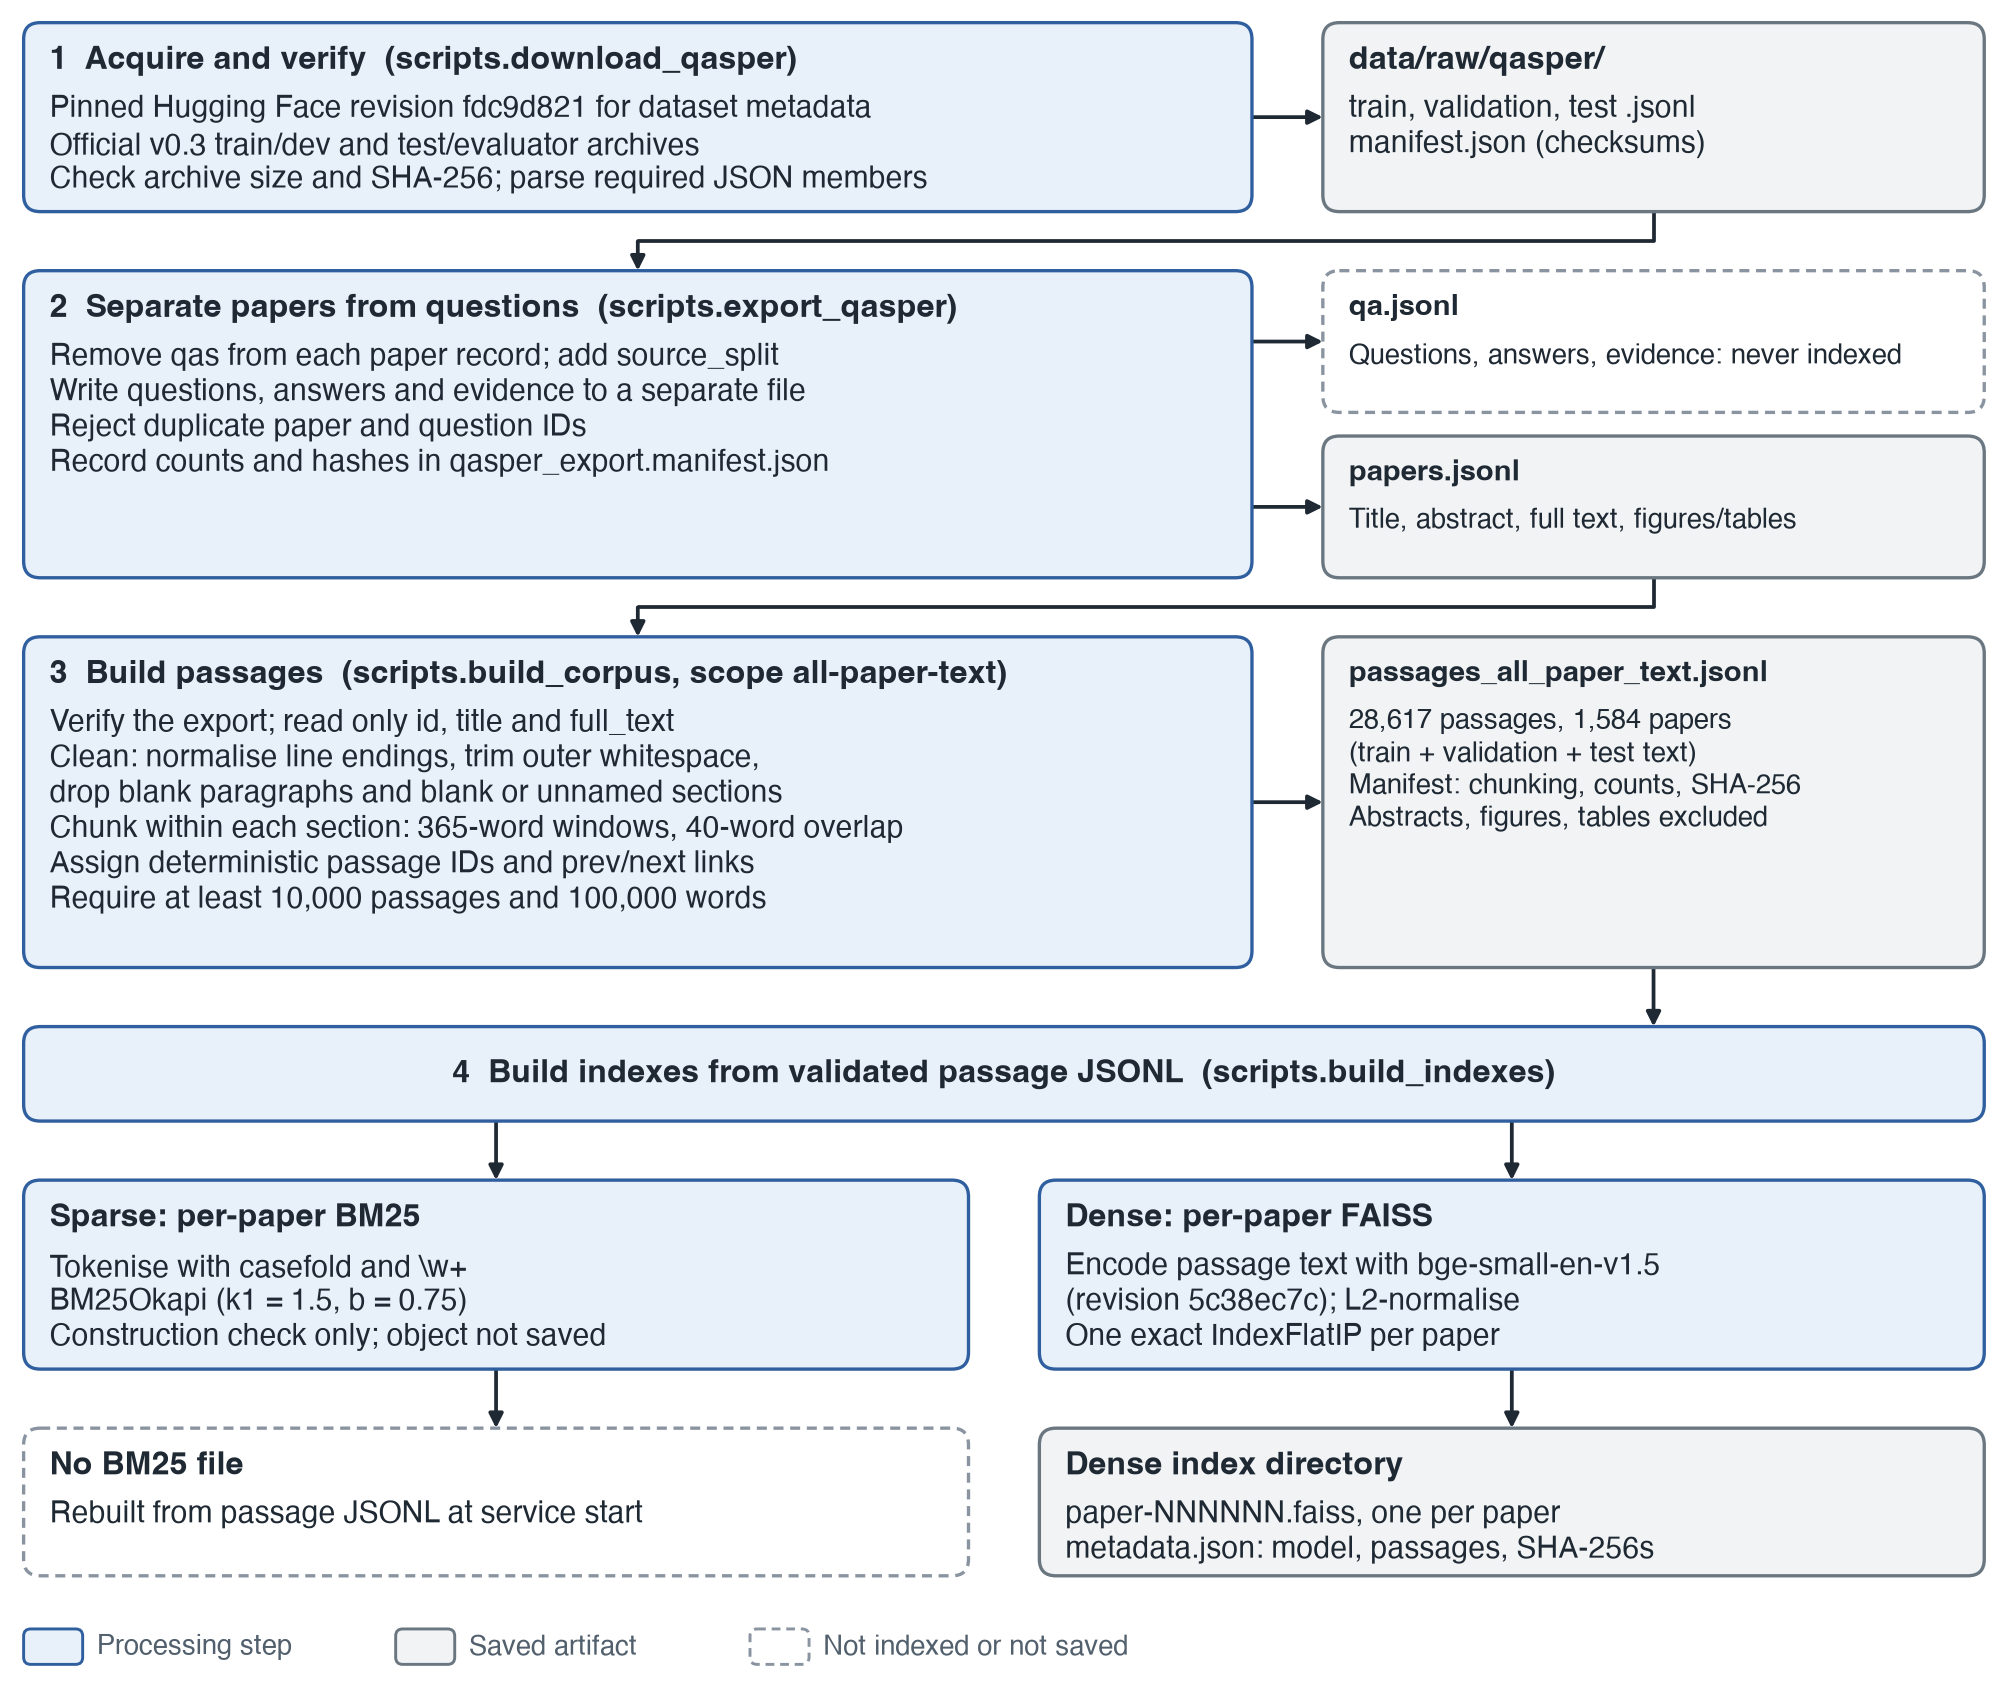
\includegraphics[width=\linewidth,height=0.78\textheight,keepaspectratio]{images/offline-corpus-index.png}
\caption{Offline corpus preparation and index construction. BM25 is reconstructed from passage JSONL when the service starts; dense indexes and their metadata are saved. Abstracts and figure/table text are excluded from the indexed passages.}\label{fig:offline}
\end{figure}


\subsection{Application and scope (Q1.2)}
PaperRAG supports researchers investigating NLP methods and findings through evidence-grounded question answering. It aims to reduce the effort of locating evidence scattered across papers and sections and tracing claims to their sources.

Users enter a natural-language question and choose either a specific paper or the full collection. Selected-paper search supports detailed questions about a paper's methods, datasets, experiments and results. Collection-wide search supports topic exploration by retrieving relevant passages across papers. The system generates an answer with inspectable passage citations, or an explicit refusal when the available evidence is insufficient. Users can open the cited passages to examine the support for individual claims.

Example inputs include:
\begin{itemize}
\item[$\bullet$] \textbf{Selected paper:} ``Which datasets are used to evaluate the proposed method?''
\item[$\bullet$] \textbf{Selected paper:} ``How does the proposed approach differ from the baselines?''
\item[$\bullet$] \textbf{Full collection:} ``What approaches are used for machine translation when parallel training data is limited?''
\item[$\bullet$] \textbf{Full collection:} ``How do entity-linking models use surrounding context to resolve ambiguous names?''
\end{itemize}

The intended benefit is to reduce the effort required to locate and inspect evidence during research. Formal evaluation uses selected-paper questions; collection-wide search is demonstrated separately in Q2.2.


\subsection{Knowledge base size (Q1.3)}
The corpus combines paper text from QASPER's training, validation and test splits. \hyperref[tab:corpus]{Table~\ref*{tab:corpus}} summarizes its size after cleaning and chunking.

\begin{table}[htbp]\centering
\caption{Corpus size for the reported 365/40 chunking configuration.}\label{tab:corpus}
\begin{tabularx}{\linewidth}{>{\hsize=1.4\hsize\linewidth=\hsize}Y>{\hsize=.6\hsize\linewidth=\hsize}Y}\toprule
Measure & Count\\\midrule
Source documents (papers) & 1,585\\
Documents with indexed chunks & 1,584\\
Indexed chunks (passages) & 28,617\\
Source-text words, excluding chunk overlap & 5,659,921\\
Words across chunks, including overlap & 5,930,961\\
Unique word types across chunks & 210,909\\\bottomrule
\end{tabularx}
\end{table}

Words are counted as whitespace-delimited units. Unique types are counted after case folding, with punctuation retained. The chunk-word total is higher because overlapping text is counted in each chunk where it appears. One source paper produces no usable chunks and is therefore absent from the index. The 28,617 chunks and 5,659,921 source-text words exceed the assignment's 10,000-passage and 100,000-word minimums.

\section{System and interface (Q2)}
\subsection{User interface (Q2.1)}


\textbf{Implementation.} We built a web interface using Streamlit, connected to the retrieval and generation pipeline through a FastAPI service. It provides a single place to ask questions and inspect the evidence supporting an answer.

\textbf{Querying.} Users select a specific paper or search across the full collection, enter a natural-language question and submit it. They can also choose an example question to get started. \hyperref[fig:ui-entry]{Figure~\ref*{fig:ui-entry}} shows the input screen with a question entered and the full collection selected.

\textbf{Inspecting results.} The interface displays the generated answer with passage citations and expandable source details. Users can inspect the cited text, evidence status and validation warnings; retrieval history provides further detail when needed. Keeping supporting information expandable makes the main answer easy to read while allowing users to investigate its evidence. \hyperref[fig:ui]{Figure~\ref*{fig:ui}} shows a returned answer and its sources.

\textbf{Interaction scope.} When the system returns a refusal, the interface presents it as an outcome rather than a technical error. Each submitted question is processed independently; displayed session history does not provide conversational memory.

\begin{figure}[htbp]\centering
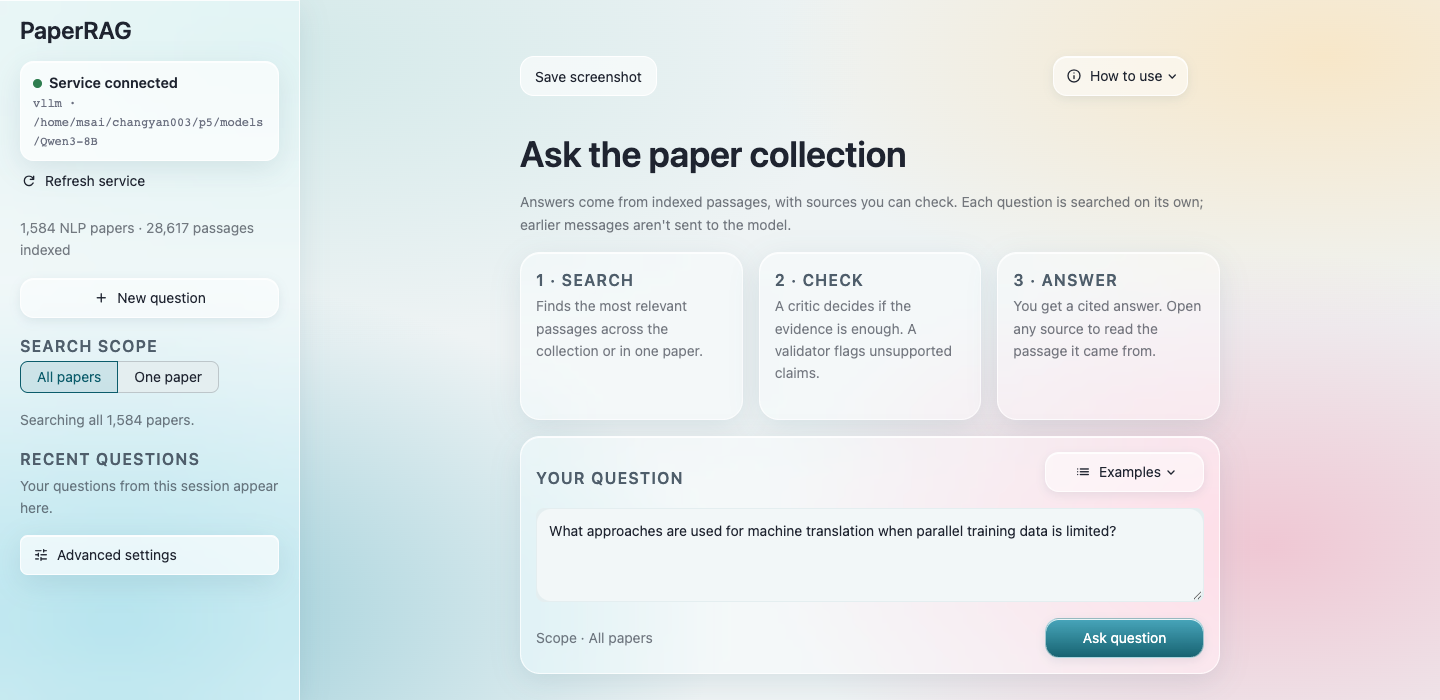
\includegraphics[width=0.97\linewidth]{figures/ui-query-entry.png}
\caption{The interface before submission, with query 3 of \hyperref[tab:queries]{Table~\ref*{tab:queries}} entered and all papers in scope. \hyperref[fig:ui]{Figure~\ref*{fig:ui}} shows the resulting answer.}\label{fig:ui-entry}
\end{figure}

\begin{figure}[htbp]\centering
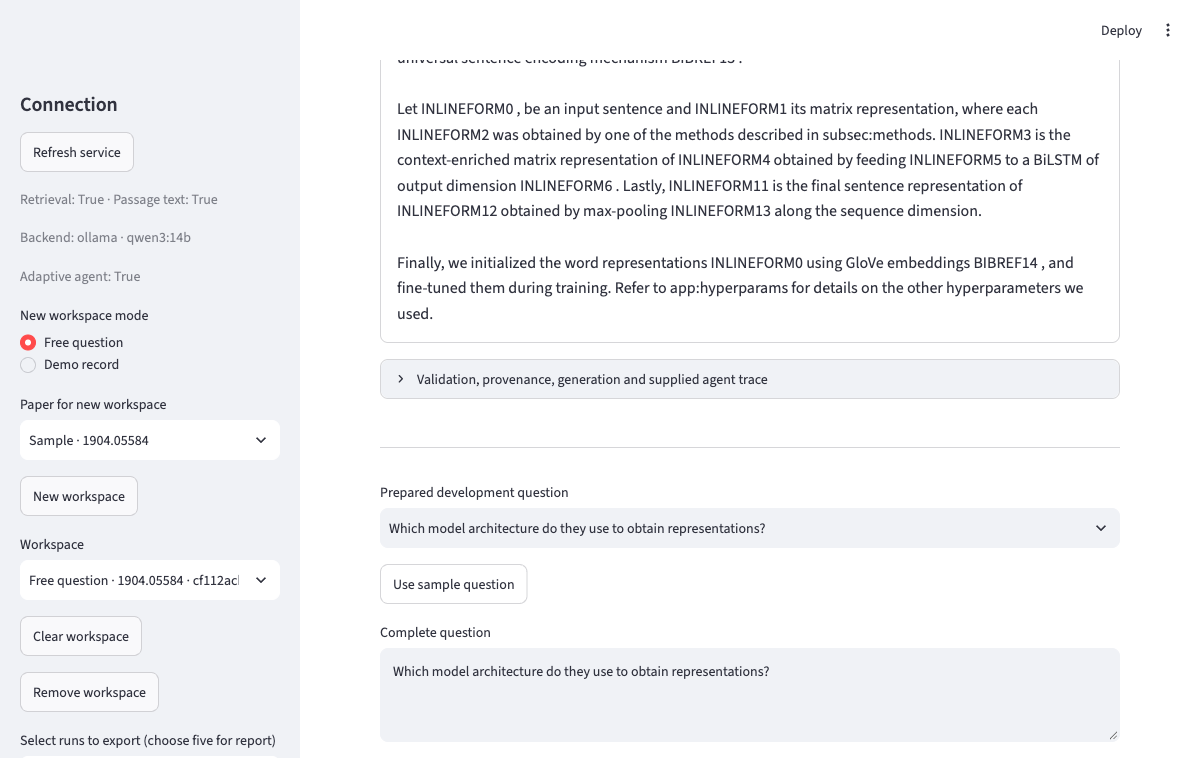
\includegraphics[width=0.97\linewidth,height=0.52\textheight,keepaspectratio]{figures/ui-answer.png}
\caption{The interface answering query 3 of \hyperref[tab:queries]{Table~\ref*{tab:queries}} in a browser against the live GPU service, with all papers in scope. The answer raised no validator warnings, and each source card shows its passage, rank and RRF score. \hyperref[fig:five-queries]{Figure~\ref*{fig:five-queries}} shows how flagged sentences appear.}\label{fig:ui}
\end{figure}

\subsection{Five measured queries (Q2.2)}\label{sec:five-queries}
\par\smallskip
\noindent\begin{minipage}{\linewidth}
\captionsetup{type=table}\small\centering
\caption{The five demonstration queries, run with all papers in scope.}\label{tab:queries}
\begin{tabularx}{\linewidth}{@{}>{\raggedright\arraybackslash}p{5mm}Y@{}}\toprule
\# & Question\\\midrule
1 & How do entity-linking models use surrounding context to resolve ambiguous names?\\
2 & How is commonsense knowledge used to improve dialogue systems?\\
3 & What approaches are used for machine translation when parallel training data is limited?\\
4 & What methods have researchers used to induce context-free grammars (CFGs)? Cite the papers supporting your answer.\\
5 & What methods are used for low-resource language identification?\\\bottomrule\end{tabularx}
\end{minipage}\par\medskip
\begin{table}[htbp]\small\centering
\caption{Summaries of generated outputs, not verified factual answers. Warning counts are validator diagnostics.}\label{tab:five-results}
\begin{tabularx}{\linewidth}{rYrrrr}\toprule
\# & Output summary & Rounds & Cites & Warnings & Seconds\\\midrule
1 & Yes; cross-language vector mapping, checked against Google Translate & 1 & 4 & 2 & 174.2\\
2 & Average classification accuracy & 3 & 1 & 2 & 98.7\\
3 & F1: 88\% on OntoNotes, 53\% on Wiki(gold) & 1 & 1 & 0 & 159.5\\
4 & BiLSTM with max pooling & 1 & 1 & 1 & 104.6\\
5 & Refused: insufficient evidence & 1 & 0 & 0 & 76.3\\\bottomrule\end{tabularx}\end{table}

\textbf{Run setup.} We submitted the five queries in \hyperref[tab:queries]{Table~\ref*{tab:queries}} through the Streamlit interface, with the full collection selected. Requests ran sequentially against the school GPU service using Qwen3-8B through vLLM and top-eight RRF retrieval without reranking. The service was already running; no dedicated warm-up query was used.

\textbf{Results.} \hyperref[tab:five-results]{Table~\ref*{tab:five-results}} summarizes the returned answers, citation counts, validation warnings and latency. \hyperref[fig:five-queries]{Figure~\ref*{fig:five-queries}} shows the corresponding interface outputs. The summaries describe generated responses; warning counts are validator diagnostics.

\textbf{Query speed.} Latency was measured as the client-observed answer HTTP response time, including retrieval, critic processing and answer generation, but excluding subsequent citation lookup and interface rendering. Mean latency was 19.9 seconds, with a median of 19.3 seconds and a range of 15.1--26.3 seconds. Query 5 took longest and required three retrieval rounds; the others required one. Each query was measured once, so these figures describe the demonstration rather than repeated-run performance.

\begin{figure}[htbp]\centering
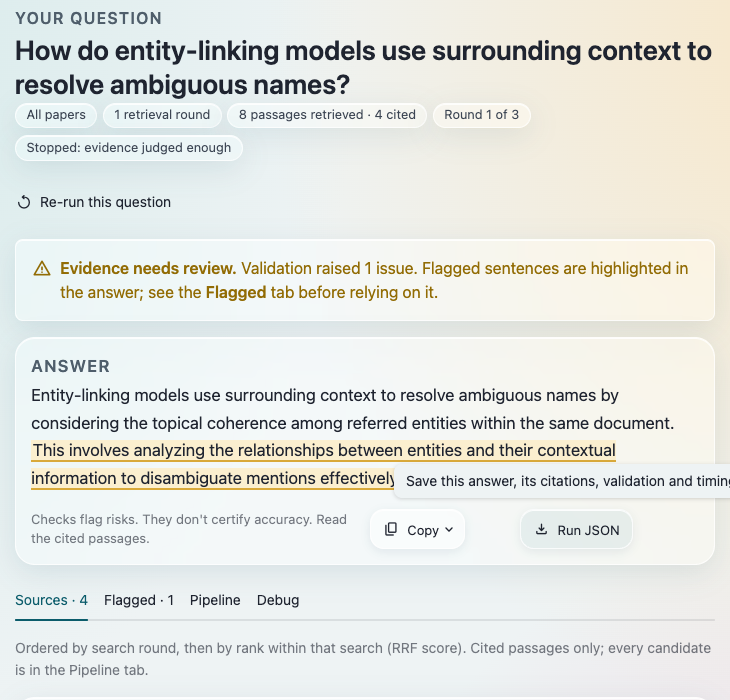
\includegraphics[width=0.48\linewidth]{figures/query-1.png}\hfill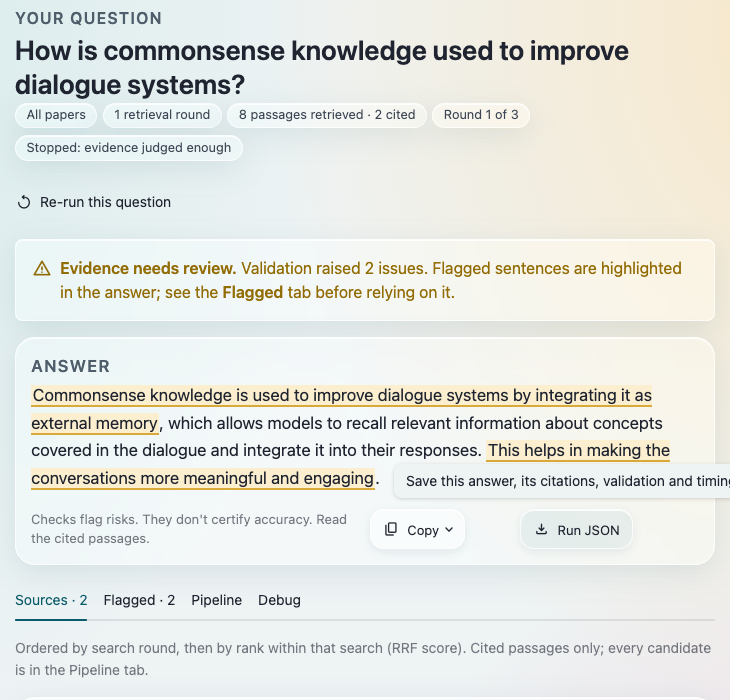
\includegraphics[width=0.48\linewidth]{figures/query-2.png}\\[2mm]
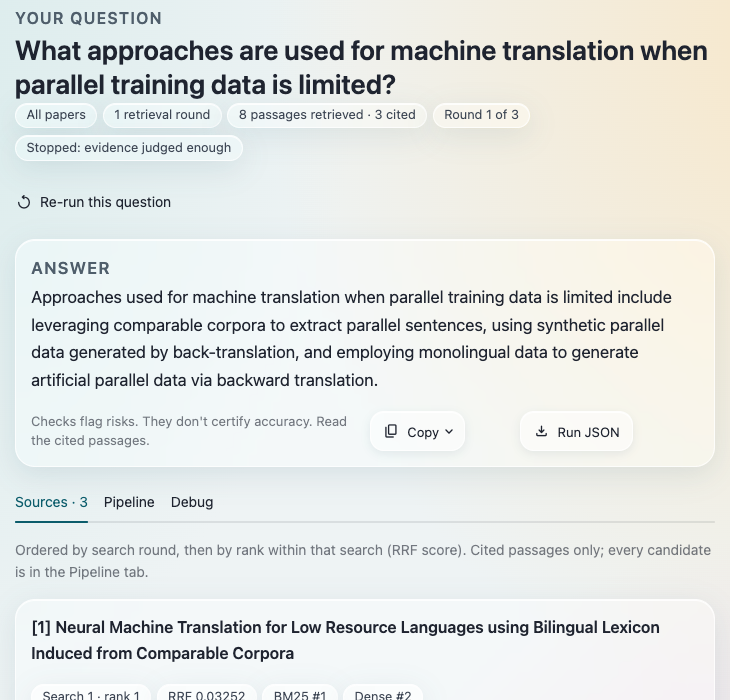
\includegraphics[width=0.48\linewidth]{figures/query-3.png}\hfill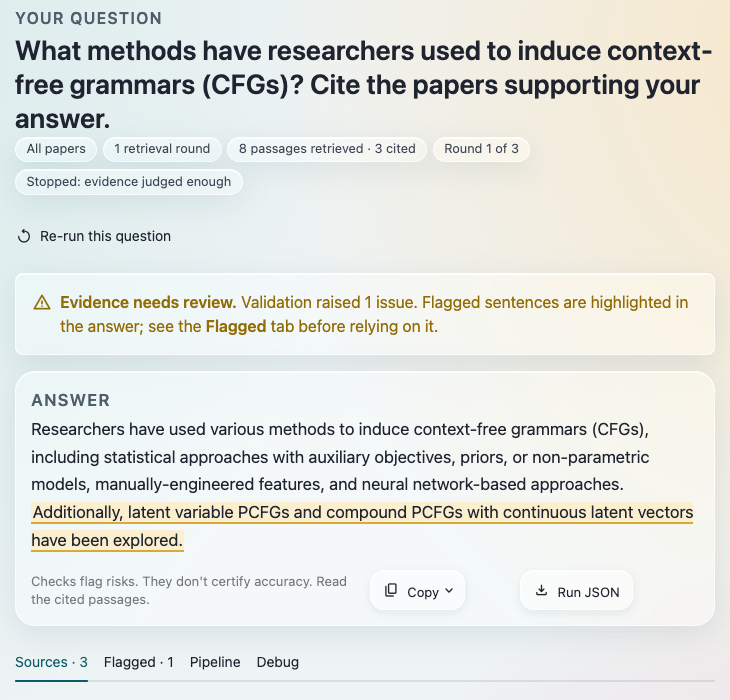
\includegraphics[width=0.48\linewidth]{figures/query-4.png}\\[2mm]
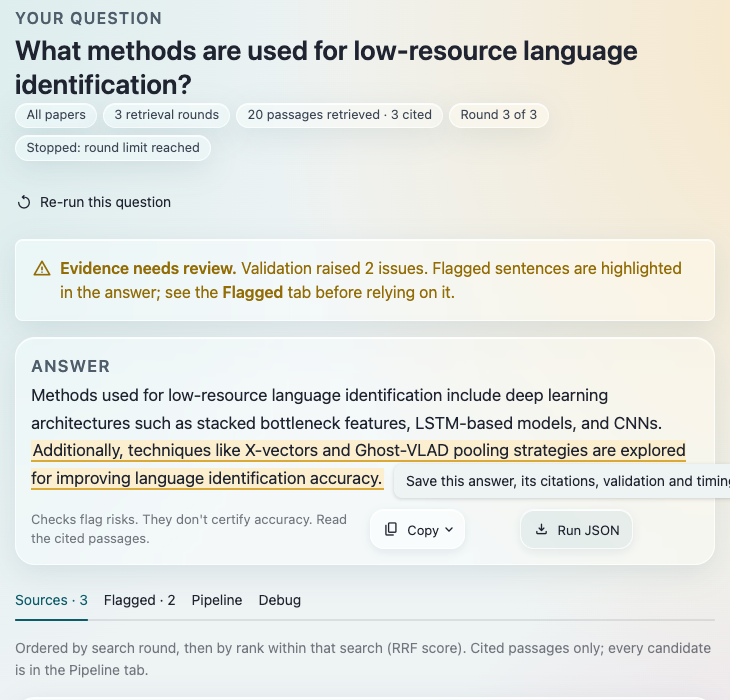
\includegraphics[width=0.48\linewidth]{figures/query-5.png}
\caption{Answers to queries 1--5 as shown by the interface, left to right and top to bottom. Screenshots are cropped to the answer column.}\label{fig:five-queries}
\end{figure}

\textbf{Result observations.} All five queries returned answers, and all 15 citations resolved to passage text. The AI-assisted inspection of cited passages found support for Query 3's listed approaches, while the other outputs contained omissions, unsupported claims or citation mismatches. Query 2's cited passages did not support its dialogue-related answer. Query 4 included a citation mismatch for compound PCFGs and did not name the supporting papers in the answer text, although source cards identified them. Query 5 illustrates the role of source inspection: the system retrieved passages ranked as relevant, but some did not directly support the associated claims. These exploratory queries demonstrate the query workflow and citation inspection; quantitative answer-quality evaluation is reported in Q4.

% Hidden from report; assessment retained in review-checks/q2-2.tex.
% \begin{review}{Q2.2: AI-suggested five-star implementation self-check}
\draftreview{P6}{P5, P4}{P6 verifies the five-query records and timing calculations; P5 checks answer support and citation behavior; P4 investigates critic mismatches.}
\aistars{4}\quad\textbf{Provisional AI assessment (7 November 2026, post-review): 4/5 stars.} This is an editorial assessment of the documented evidence, not a course grade or human sign-off. Five all-papers queries have inputs, output summaries, rounds, citation and warning counts, timings and screenshots. The prose checks grounding against cited passages and identifies confident unsupported answers, including critic/generator disagreement. Hardware and timing boundaries are stated. One serial pass without reference answers cannot estimate accuracy or latency variability; the run export does not fix the job identifier or passage budget, and the AI-assisted grounding check still needs P5/P4 confirmation.
\end{review}


\section{Retrieval design and experiments (Q3)}
\subsection{Retrieval problems and design}
Scientific questions may use different wording from the passages that answer them, while exact dataset and model names remain important. We combine lexical and dense retrieval to address these complementary matching needs. Reranking tests whether joint query--passage scoring improves candidate ordering, while chunk-size and retrieval-depth experiments examine the trade-off between evidence coverage and the amount of text supplied.

\textbf{Complementary retrieval.} BM25 \citep{robertson2009bm25} uses term matching with term-frequency saturation and passage-length normalization. Our implementation applies case folding and Unicode word-token extraction, with $k_1=1.5$ and $b=0.75$. Dense retrieval uses \texttt{BAAI/bge-small-en-v1.5} \citep{baai2023bgesmallv15} to encode queries and passages, ranking L2-normalized vectors through per-paper FAISS exact inner-product search. A search instruction is prepended to queries only. Evaluation ranks passages within the selected paper.

\textbf{Hybrid fusion.} Each retriever returns up to 20 candidates. We deduplicate by passage ID and combine rankings using reciprocal rank fusion \citep{cormack2009rrf}:
\begin{equation}
\operatorname{RRF}(p)=\sum_{s:p\in L_s}\frac{1}{60+\operatorname{rank}_s(p)}.
\end{equation}
Ranks start at one; a passage absent from a list contributes nothing for that source. Fusion combines lexical and vector rankings without assuming their scores have comparable scales.

\textbf{Reranking and input limits.} We tested \texttt{BAAI/bge-reranker-base}, a cross-encoder that jointly scores each query and passage, on the fused candidate union. The dense encoder limits each encoded input to 512 tokens; the reranker applies a 512-token limit to the combined query--passage input. In the reported corpus, 14.3\% of passages exceed the dense encoder's limit; BM25 reads their full text. This may affect which evidence is represented, but its effect on retrieval quality was not isolated. Generation-side clipping is discussed in Q4.2.

\hyperref[fig:hybrid]{Figure~\ref*{fig:hybrid}} shows the retrieval branches, fusion, evidence pool and retry path.
\begin{figure}[htbp]\centering
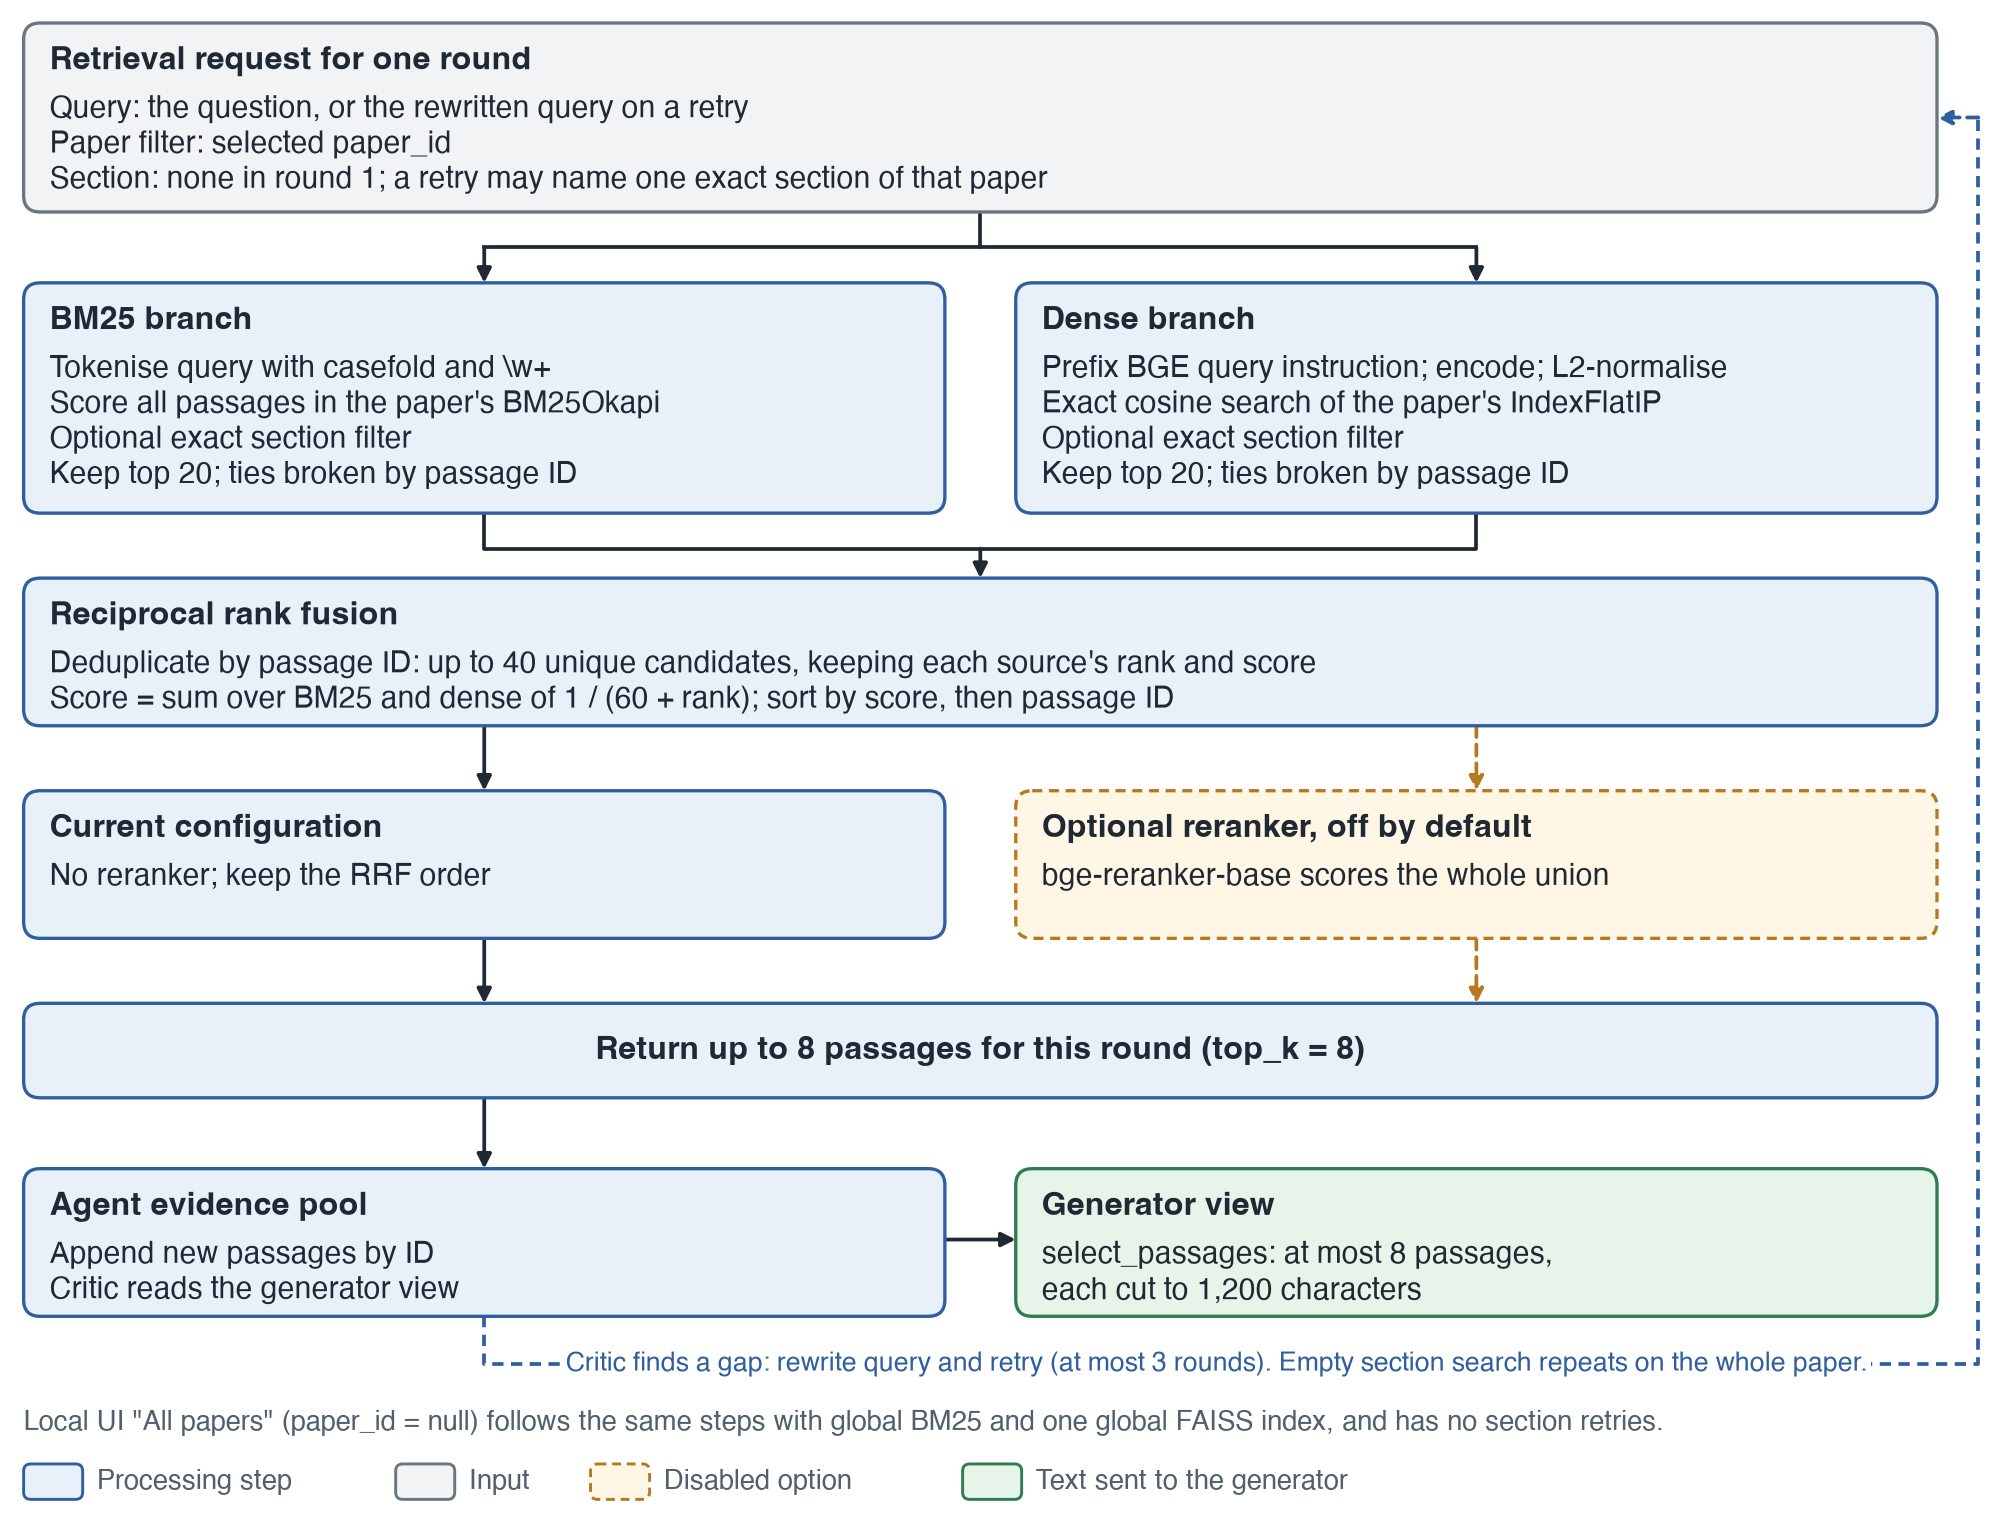
\includegraphics[width=\linewidth,height=0.78\textheight,keepaspectratio]{images/online-hybrid-retrieval.png}
\caption{Online hybrid retrieval and the bounded retry loop. The current configuration returns up to eight RRF passages per round without reranking; the optional reranker is shown as a disabled comparison. The critic and generator use the same clipped evidence view. This top-eight agent setting is separate from the reported retrieval evaluation at $K=5$.}\label{fig:hybrid}
\end{figure}


\subsection{Evaluation setup and rank-aware results}
% Generated from results/p6/retrieval-draft-v3/summary.json
\begin{table}[htbp]\centering
\caption{Development retrieval on draft labels. Recall and nDCG are relative to the judged pool.}\label{tab:retrieval}
\begin{tabular}{lrrrr}\toprule
Method & P@5 & Pool R@5 & MRR@5 & Pool nDCG@5\\\midrule
BM25 & 0.482 & 0.607 & 0.730 & 0.636\\
Dense & 0.527 & 0.698 & 0.799 & 0.719\\
Hybrid RRF & 0.539 & 0.714 & 0.804 & 0.731\\
RRF + reranker & 0.509 & 0.659 & 0.718 & 0.663\\\bottomrule\end{tabular}\end{table}

The frozen ranking pool contains four methods for 200 questions, evaluated against the accepted binary question--passage label file. \hyperref[tab:retrieval]{Table~\ref*{tab:retrieval}} reports scores from the accepted-label run. Precision@5 measures relevant results among the five returned slots; MRR@5 rewards an early first relevant passage. Pool-relative recall measures recovery of the relevant passages that were judged, not every relevant passage in the paper. Binary nDCG discounts relevant passages by rank and normalizes against the ideal ranking within the judged pool.

The judged pool is the deduplicated union of the four methods' saved top-five results, comprising 1,853 question--passage pairs. All scored top-five results are judged. Scores are macro-averaged with equal weight per question: precision and MRR use 200 questions, while pool recall and nDCG exclude one question with no positive labels, leaving 199. The pool is not exhaustive: relevance outside it remains unknown, so scoring other methods or deeper cutoffs may require additional judgments.

RRF achieves the highest mean scores in \hyperref[tab:retrieval]{Table~\ref*{tab:retrieval}}. The paired comparisons below assess whether its differences from the other methods are consistent across questions. Annotation provenance and its limitations are described in Section~\ref{sec:annotation}.

\subsubsection{Fusion and reranking comparisons at \texorpdfstring{$K=5$}{K=5}}
\begin{table}[htbp]\centering\small
\caption{Fusion and reranking comparisons at $K=5$. Differences are the first method minus the second. Intervals use 1,000 paper-cluster bootstrap resamples, seed 42, over 174 papers.}\label{tab:p2-paired}
\begin{tabularx}{\linewidth}{YYrrl}\toprule
Comparison & Metric & Difference & $n$ & 95\% interval\\\midrule
RRF -- BM25 & Precision & +0.0570 & 200 & [+0.0354, +0.0788]\\
RRF -- BM25 & Pool recall & +0.1070 & 199 & [+0.0663, +0.1471]\\
RRF -- BM25 & MRR & +0.0747 & 200 & [+0.0398, +0.1112]\\
RRF -- BM25 & Pool nDCG & +0.0958 & 199 & [+0.0640, +0.1273]\\
RRF -- Dense & Precision & +0.0120 & 200 & [-0.0063, +0.0318]\\
RRF -- Dense & Pool recall & +0.0161 & 199 & [-0.0139, +0.0462]\\
RRF -- Dense & MRR & +0.0052 & 200 & [-0.0330, +0.0434]\\
RRF -- Dense & Pool nDCG & +0.0125 & 199 & [-0.0154, +0.0409]\\
RRF+BGE -- RRF & Precision & -0.0300 & 200 & [-0.0555, -0.0051]\\
RRF+BGE -- RRF & Pool recall & -0.0550 & 199 & [-0.1037, -0.0098]\\
RRF+BGE -- RRF & MRR & -0.0868 & 200 & [-0.1377, -0.0350]\\
RRF+BGE -- RRF & Pool nDCG & -0.0682 & 199 & [-0.1123, -0.0256]\\
\bottomrule\end{tabularx}\end{table}

\hyperref[tab:p2-paired]{Table~\ref*{tab:p2-paired}} uses paired question scores and 1,000 paper-cluster bootstrap resamples (seed 42). Each resample draws 174 papers with replacement, retains their valid question pairs, and computes the question-weighted mean difference; endpoints are the 2.5th and 97.5th percentiles. Precision/MRR use 200 questions, and pool recall/nDCG use 199. RRF improves on BM25 across all four metrics, with all intervals above zero. RRF has only small gains over Dense; intervals that include zero do not establish a reliable improvement. The tested reranker produces lower aggregate scores than RRF across all four metrics; its unadjusted paired intervals are below zero. These are 12 exploratory comparisons without multiple-comparison correction, and the intervals do not account for annotation bias. The results therefore describe this evaluated pool rather than a general ordering of retrieval methods.

The four-method comparison is evaluated at $K=5$. The agent's top-eight RRF configuration was selected separately using development evidence-recall results, discussed below.

\subsubsection{Paired BM25--Dense comparison at \texorpdfstring{$K=5$}{K=5}}
% Means: results/p2-final-retrieval-handoff/scored/retrieval.csv.
% Paired differences and intervals: results/p1-bm25-vs-dense-verification-20261105/comparison/ablation.csv.
% Differences use the unrounded per-question scores, not rounded table means.
\begin{table}[htbp]\centering\small
\caption{BM25 versus Dense at $K=5$ on the accepted relevance labels. Differences are Dense minus BM25. Percentile intervals use 1,000 paper-cluster bootstrap resamples, seed 42; all rows cover 174 papers. $n$ denotes questions.}\label{tab:bm25-dense-paired}
\begin{tabularx}{\linewidth}{Yrrrrl}\toprule
Metric & BM25 & Dense & Difference & $n$ & 95\% interval\\\midrule
Precision & 0.4820 & 0.5270 & $+0.0450$ & 200 & [0.0171, 0.0728]\\
Pool recall & 0.6067 & 0.6976 & $+0.0909$ & 199 & [0.0419, 0.1421]\\
MRR & 0.7296 & 0.7992 & $+0.0696$ & 200 & [0.0168, 0.1222]\\
Pool nDCG & 0.6355 & 0.7188 & $+0.0833$ & 199 & [0.0366, 0.1314]\\\bottomrule
\end{tabularx}
\end{table}

Dense has higher mean scores than BM25 on all four metrics in this judged pool. The Precision@5 gain of 4.50 percentage points corresponds to an average of 0.225 additional passages labelled relevant per question among the five returned slots. Pool recall improves by approximately 9.09 percentage points. These results favour Dense over BM25 as a single-retriever quality baseline for this fixed evaluation at $K=5$; downstream answer quality is not measured here.

\hyperref[tab:bm25-dense-paired]{Table~\ref*{tab:bm25-dense-paired}} uses the same paper-cluster bootstrap procedure and metric denominators as the fusion comparisons. All four intervals are above zero. These findings are conditional on the evaluated questions and accepted labels; pool-relative recall is not exhaustive paper-level recall.

\subsection{Illustrative query comparisons}
\paragraph{Complementary BM25 and Dense results.}
The examples below illustrate contrasting outcomes within the evaluated pool. They use the accepted relevance labels and were selected to explain ranking behavior, not to estimate its frequency or establish generated-answer correctness.

For ``Which commonsense knowledge base are they using?'' (paper \texttt{1709.05453}; \citep{young2017dialog}), Dense retrieves both passages labelled relevant at ranks one and five; BM25 retrieves neither in its saved top five. The rank-five passage states, ``In our experiment, ConceptNet is used as the commonsense knowledge base.'' Dense's precision is 0.4 and pool recall is 1.0, compared with zero for BM25 on both metrics. This illustrates the evidence retrieved by Dense at the evaluated cutoff; the cause of the ranking difference was not isolated.
% Question 042800c3336ed5f4826203616a39747c61382ba6. Exact passage IDs: review-checks/p1-evidence.md.

For ``What baselines do they propose?'' (paper \texttt{2003.12660}; \citep{ahia2020pidgin}), BM25 retrieves relevant passages at ranks three and five describing supervised and unsupervised translation baselines, tokenization variants and their architecture. The rank-five passage states, ``All baseline models were trained using the Transformer architecture''. The rank-five hit has a BM25 score of zero and is ordered by passage ID among ties, so its inclusion should not be interpreted as a strong lexical match. Dense retrieves no passage labelled relevant in its saved top five. BM25's precision is 0.4 and pool recall is 0.5, compared with zero for Dense on both metrics. Dense's fourth and fifth passages mention supervised and unsupervised models, but are labelled non-relevant in the accepted labels. The example illustrates query-specific complementarity under the recorded judgments: Dense's higher aggregate scores do not mean that it retrieves more relevant evidence for every question.
% Question dd81f58c782169886235c48b8f9a08e0954dd3ae. Exact passage IDs: review-checks/p1-evidence.md.

\paragraph{Contrasting effects of reranking.}
For ``How effective is their NCEL approach overall?'' (paper \texttt{1811.08603}; \citep{cao2018ncel}), RRF returns the three pool passages labelled relevant at ranks one, three and four. The rank-one passage describes NCEL outperforming baselines on both easy and hard entity-linking datasets; the rank-three passage gives a concrete disambiguation example, and rank four summarizes evaluation across five benchmarks. BGE retains only the last of these at rank four in its top five. RRF precision/pool recall are 0.6/1.0, versus 0.2/0.3333 after reranking. The relevant evidence excluded from BGE's top five is known from the saved outputs; its exact lower ranks are not available. This example illustrates a change in the top-five evidence set; it does not identify the cause.
% Question 114934e1a1e818630ff33ac5c4cd4be6c6f75bb2; passage IDs: review-checks/p2-evidence.md.


The rank-three NCEL passage is a debatable relevance judgment for overall effectiveness. Even excluding that passage from both methods, RRF retains two accepted relevant passages versus one with BGE. The published scores retain the accepted gold unchanged.

\paragraph{A contrasting reranking improvement.}
For ``what are the state of the art models?'' (paper \texttt{1803.09000}), reranking increases Precision@5 from 0.2 to 0.4 under the accepted labels, although MRR@5 falls from 0.5 to 0.3333 because its first relevant passage moves from rank two to rank three. The precision gain depends on one passage whose two annotators disagreed and whose final label was resolved during review. This illustrates a query-specific precision gain alongside a lower reciprocal rank, despite the reranker's lower aggregate scores.
% Question d7799d26fe39302c4aff5b530aa691e8653fffe8; source: pinned P2 scores.jsonl, rankings and accepted labels.


\subsection{Chunk size and retrieval depth}
We compared BM25 chunk sizes through a coarse-to-fine search, holding overlap at 40 words and retrieval within the question's paper. Initial experiments on 50 questions narrowed the candidates to 325, 365 and 375 words. A final comparison used 200 additional questions fixed before retrieval. All 250 selection questions were excluded from the final relevance evaluation.

The comparison uses questions whose supporting evidence can be fully and unambiguously located in the paper text. An evidence hit means that the retrieved text jointly covers at least one complete annotated evidence paragraph; complete evidence means covering every supporting paragraph for at least one reference answer. We compare coverage under fixed reading budgets of 500, 1,000 and 2,000 words, counting overlapping text each time it appears and cutting the final passage to fit. Top-five coverage is supplementary because larger chunks also supply more text.

On the 200 additional questions, 365-word chunks give slightly higher top-five coverage than 375-word chunks: 147 versus 145 evidence hits and 125 versus 123 complete-evidence successes. They also require slightly less reading (1,247 versus 1,262 words on average). However, under the primary 1,000-word budget, 375 words covers complete evidence for 108 questions versus 106 for 365; at 500 words, 325 performs best with 75 successes. We chose 365/40 as a compromise between coverage and reading volume. Overlap was held fixed rather than tuned.

A separate agent development slice contains 40 questions, of which 32 have mapped evidence. Static RRF evidence recall rises from 0.740 at top five to 0.885 at top eight and 0.974 at top ten. Complete evidence is recovered for 22, 26 and 30 of the 32 questions, respectively. These are mapped-evidence metrics, distinct from relevance-pool recall in \hyperref[tab:retrieval]{Table~\ref*{tab:retrieval}}. Top eight matches the generator's passage-count limit; top ten is a retrieval diagnostic and exceeds that limit.
The frozen downstream evaluation supplies a separate depth analysis on 200 questions with 347 mapped gold passages, using one saved ranking per question. Plain retrieval recovers 0.723 of the mapped evidence at five passages, 0.858 at eight, 0.897 at ten and 0.953 at fifteen (\hyperref[tab:depth]{Table~\ref*{tab:depth}}). The ordering matches the development slice, but the curve is flatter: ten passages recover 0.897 here against 0.974 on the slice, showing that the size of the depth gain varies between question sets. The eight-passage setting was chosen on development evidence and was not changed afterwards. Because the agent developer labelled 40 of these questions for annotation before the freeze, we also report the remaining 160; both subsets show increasing recall with depth. Mapped-evidence recall differs from the pool-relative recall of \hyperref[tab:retrieval]{Table~\ref*{tab:retrieval}}.
\begin{table}[htbp]\centering\small
\caption{Mean mapped gold recall of plain retrieval by depth (no critic, no retry); complete evidence in brackets. Held-out depths come from one 15-passage ranking. ``160 not annotated'': held-out questions the agent developer did not annotate.}\label{tab:depth}\vspace{1.5mm}
\begin{tabularx}{\linewidth}{>{\hsize=1.8\hsize\linewidth=\hsize}Y>{\hsize=0.84\hsize\linewidth=\hsize}Y>{\hsize=0.84\hsize\linewidth=\hsize}Y>{\hsize=0.84\hsize\linewidth=\hsize}Y>{\hsize=0.84\hsize\linewidth=\hsize}Y>{\hsize=0.84\hsize\linewidth=\hsize}Y}\toprule
Questions & Top 3 & Top 5 & Top 8 & Top 10 & Top 15\\\midrule
Development slice (32) & 0.599 (17) & 0.740 (22) & 0.885 (26) & 0.974 (30) & 0.974 (30)\\
Held-out, all 200 & 0.569 (84) & 0.723 (117) & 0.858 (154) & 0.897 (166) & 0.953 (183)\\
Held-out, 160 not annotated & 0.585 (69) & 0.749 (98) & 0.881 (127) & 0.907 (134) & 0.959 (148)\\\bottomrule\end{tabularx}
\end{table}
\begin{figure}[htbp]\centering
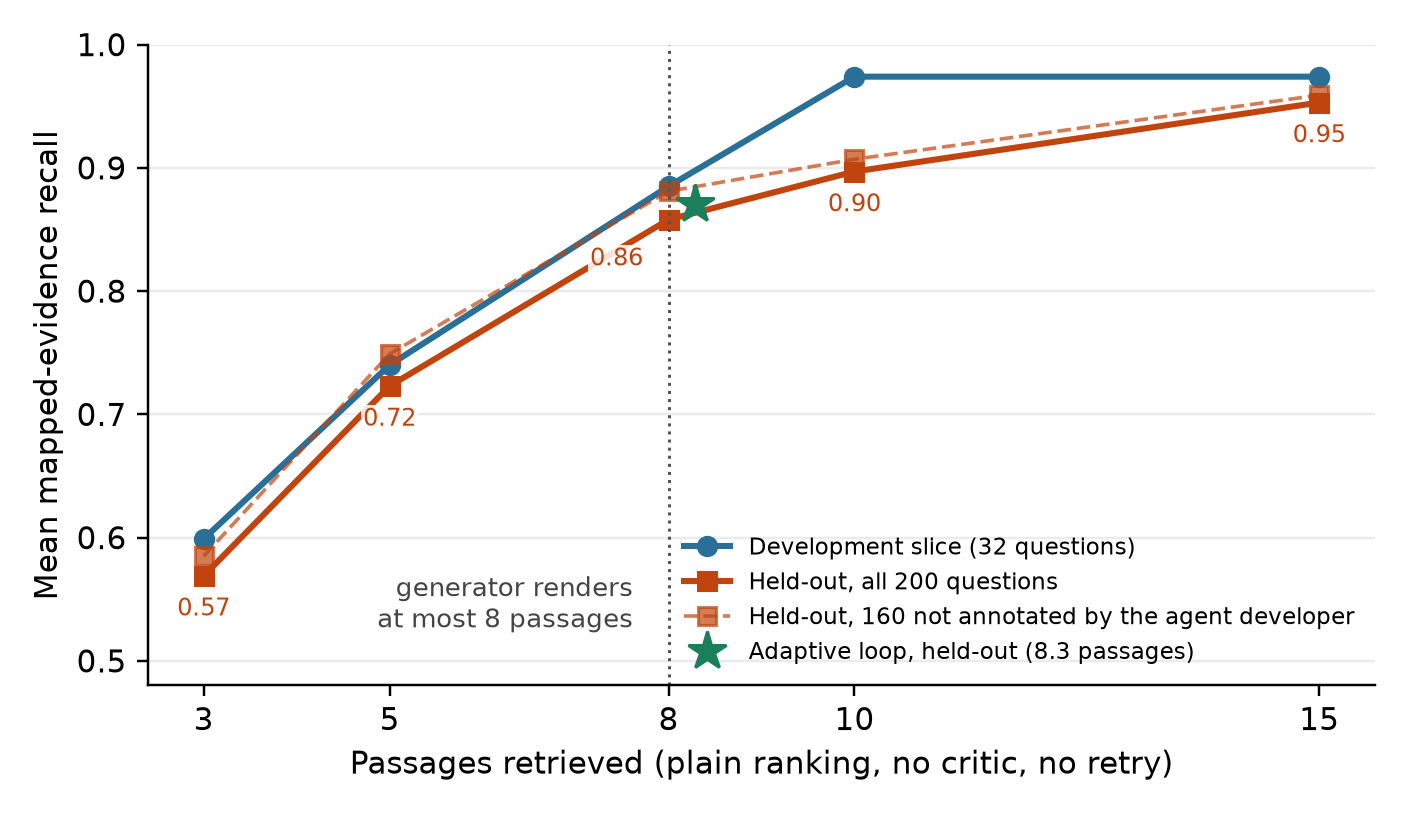
\includegraphics[width=0.92\linewidth]{images/recall-by-depth.png}
\caption{Mean mapped-evidence recall of plain retrieval by depth (the values of \hyperref[tab:depth]{Table~\ref*{tab:depth}}). The development slice reaches 0.974 at ten passages, the held-out curve is flatter (0.897 at ten), and the adaptive result on the held-out questions (star) is close to plain retrieval at a comparable passage budget. The generator renders at most eight passages.}\label{fig:depth}
\end{figure}
\paragraph{Evidence recovered by increasing depth.} For ``Where did they get the data for this project?'' (development paper \texttt{1805.11535}; reference answer: Twitter), the passage labelled as evidence is ranked seventh. It states, ``Our dataset is constructed via distant supervision from Twitter.'' Top-five retrieval excludes it, whereas top eight includes it. The 599-character passage fits within the generator's context limit. This is a concrete improvement in evidence access; the generated answer cites a different passage, so the example does not establish an answer-grounding improvement.

\subsection{Resulting retrieval configuration}
RRF combines complementary rankings and improves on BM25 across the evaluated metrics, while its gains over Dense are small and uncertain. The tested reranker offers no aggregate benefit on this pool, although individual queries show gains. We therefore retain RRF without reranking. The 365/40 chunk configuration balances evidence coverage and reading volume; top eight was selected using development evidence and matches the generator's passage limit. Deeper rankings measure retrieval coverage beyond the rendered context, rather than evidence actually used by generation. The effects of adaptive query rewriting and its downstream ablations are reported in Q5.

% Assessment retained internally; 5/5 review boxes are hidden.
% \begin{review}{Q3: AI-suggested five-star implementation self-check}
\draftreview{P2}{P1, P3, P4, P6}{P2 leads fusion/reranking results; P1 checks sparse/dense comparisons; P3 checks chunking and gold; P4 checks depth results; P6 cross-checks scoring and tables.}
\colorbox{yellow!45}{\strut\textbf{DONE FOR DRAFT --- P1}}\par
Approved by Junlin Yin on 6 November 2026 for the BM25/Dense methods, paired comparison and two contrasting examples. Other owners' reviews remain pending.\par\smallskip
\textbf{P2 technical checks complete; owner approval pending.}\par Numerical comparisons and examples checked against saved outputs; Vishakha must confirm final wording before replacing this with an owner sign-off.\par\smallskip
\aistars{3}\quad\textbf{Provisional AI assessment: 3/5 stars. Target: 5/5 --- strong implementation.} This is an editorial assessment, not a course grade. Sparse, dense, hybrid and reranked comparisons are implemented, and the negative reranking result is reported clearly. Accepted-label results and the independently reproduced BM25--Dense paired intervals are now included. P1's contrasting examples have been confirmed by Junlin Yin; P2 paired comparisons and a traceable reranking failure example are now incorporated; member sign-off on final wording remains pending. Confirm evaluation roles and the fusion/depth example, preserve the different denominators, and distinguish pool-relative relevance recall from mapped-evidence recall. Confirm that explanations for reranker failure remain hypotheses unless tested. This P1 approval does not complete owner sign-off for the whole Q3 section.
\end{review}


\section{Generation and evaluation (Q4)}
\subsection{Generation approach (Q4.1)}
\textbf{Task fit.} We use evidence-conditioned generative question answering because questions about scientific papers may require combining methods, datasets and findings described across several passages. A generative model can synthesize this information into a coherent response, whereas a single-span extractive approach restricts the answer to a contiguous text segment.

\textbf{Relationship to established research.} Our approach follows retrieval-augmented generation: relevant passages are retrieved from an external collection and supplied as context for answer generation \citep{lewis2020rag}. This connects the answer to accessible source material rather than relying solely on knowledge stored in model parameters. PaperRAG applies this principle through its hybrid retriever and passage-level citation interface; it does not reproduce the original RAG paper's jointly trained architecture.

Work on grounded generation also distinguishes answer correctness from citation support: ALCE evaluates both, motivating our inspectable citations and separate answer-quality and grounding measurements \citep{gao2023alce}. Self-RAG learns adaptive retrieval and critique through special reflection tokens \citep{asai2023selfrag}. PaperRAG instead uses a prompted generator, a separate bounded critic and programmatic validation, without task-specific model training. This modular design lets us change retrieval and checking policies and compare their contributions while keeping the generator fixed. It trades a learned, integrated control mechanism for explicit, separately testable stages.

\textbf{Model choice.} We selected the open-weight \texttt{Qwen/Qwen3-8B} model for deployment on the available university GPU and for control over prompts, inference settings and output processing. Qwen3 supports both thinking and non-thinking modes \citep{qwen2025}; our configuration uses non-thinking generation for direct, context-conditioned answers. This is a practical model choice for the project rather than a claim that it outperforms alternative generators.

\textbf{Evidence inspection.} The generator receives retrieved passages, a closed list of citable passage IDs and an instruction to refuse when evidence is insufficient. Structured output records the answer, citations and claim provenance. Post-generation checks assess citation validity, numerical grounding and provenance consistency, making potential support issues visible to users. These checks support inspection; semantic grounding is evaluated separately through the answer-quality and RAG metrics in Q4.4--Q4.5.

\textbf{Primary evaluation configuration.}
\begin{center}\small
\begin{tabularx}{\linewidth}{lY}\toprule
Model serving & Qwen3-8B, vLLM 0.11.0, bfloat16, one NVIDIA A40 (46\,GB)\\
Decoding & Greedy (temperature 0), top-$p$ 0.9, thinking disabled; up to 1,024 new tokens\\
Context & 32,768-token model limit; up to eight passages of 1,200 characters each\\
Prompt & \texttt{p5-grounded-qa-v7}\\\bottomrule
\end{tabularx}
\end{center}

% 5/5 assessment retained internally.
% \begin{review}{Q4.1: AI-suggested five-star implementation self-check}
\draftreview{P5}{P4, P6}{P5 verifies generation choices, model/prompt settings and grounding claims; P4 checks the critic/generator boundary; P6 checks citation and report consistency.}
\colorbox{yellow!45}{\strut\textbf{DONE FOR DRAFT --- P5}}\par
Approved by Junyu Hu on 6 November 2026 for the generation approach, final serving/decoding settings and grounding description. The Qwen3-8B Hub revision remains open; P4 and P6 reviews remain pending.\par\smallskip
\aistars{3}\quad\textbf{Provisional AI assessment (7 November): 3/5 stars. Target: 5/5 --- strong implementation.} This is an editorial assessment of the current evidence, not a course grade. Lowered from 4: the handout asks for the choice to be motivated in relation to the state of the art, and this section gives only a short rationale and states that no external comparison was made. Serving, decoding and prompt settings are recorded. Two stars are withheld: P5 should add a cited comparison with alternative generation approaches, and the Qwen3-8B Hub revision is unpinned with P4/P6 reviews pending.
\end{review}


\subsection{Preprocessing (Q4.2)}
\textbf{Conservative text cleaning.} QASPER provides structured paper text, so extensive microtext normalization is unnecessary. We normalize line endings, trim surrounding whitespace and remove empty content, as described in Q1.1. We retain scientific terminology, punctuation, formulas and citation placeholders to avoid changing the meaning of the evidence. Placeholders remain as supplied by the dataset; preprocessing does not reconstruct their original contents.

\textbf{Retrieval representations.} BM25 applies case folding and word-token extraction to support lexical matching. The dense encoder uses its own tokenizer and a query-specific search instruction. These transformations prepare representations for retrieval without modifying the stored passage text shown to users. Encoder inputs are limited to 512 tokens; Q3 discusses the resulting coverage considerations.

\textbf{Generation input preparation.} Retrieved passages are rendered with their citation identifiers so that generated claims can be traced to their sources. The primary evaluation supplies at most eight passages, each limited to 1,200 characters, to bound the context supplied to the generator. The critic uses the same rendered evidence view. This preparation preserves traceability and keeps the two stages' evidence consistent. Truncation can exclude useful sentences from otherwise relevant passages; the post-hoc context-budget analysis in Section~\ref{sec:context} examines a larger 2,500-character limit.

\textbf{Output postprocessing.} Generated JSON is parsed into the answer-and-citation structure. Limited repair of invalid escape sequences handles formatting irregularities before validation. Citation and grounding checks are then applied separately; formatting repair does not establish factual correctness.

% 5/5 assessment retained internally.
% \begin{review}{Q4.2: AI-suggested five-star implementation self-check}
\draftreview{P3}{P1, P5, P4}{P3 checks corpus preprocessing; P1 checks lexical/dense transformations; P5 checks prompt rendering and output parsing; P4 verifies the clipping analysis.}
\colorbox{yellow!45}{\strut\textbf{DONE FOR DRAFT --- P1}}\par
Approved by Junlin Yin on 6 November 2026 for lexical and Dense preprocessing. Other owners' reviews remain pending.\par\smallskip
\colorbox{yellow!45}{\strut\textbf{DONE FOR DRAFT --- P5}}\par
Approved by Junyu Hu on 6 November 2026 for prompt rendering (eight passages at 1,200 characters) and structured-output parsing. Corpus preprocessing is covered by the P3 box below and the P4 review remains pending; the clipping figures (73.3\%, 33 of 45 development gold passages; 66.9\%, 232 of 347 held-out gold passages) were recomputed by P4 on the final corpus.\par\smallskip
\colorbox{yellow!45}{\strut\textbf{DONE FOR DRAFT --- P3}}\par
P3 scope: stored-text normalization and preserved source placeholders checked. Prompt clipping and parsing remain for P4/P5 verification; the clipping statistic was recomputed by P4 (73.3\%, 33 of 45 development gold passages).\par\smallskip
\aistars{5}\quad\textbf{Provisional AI assessment (7 November 2026, reassessed after preprocessing revision): 5/5 stars.} This is an editorial assessment of Q4.2 requirement coverage, not a course grade or human sign-off. The section explains why structured scientific text needs conservative cleaning rather than extensive microtext normalization. It identifies the transformations applied, the scientific content retained and the distinction between stored passages and retrieval representations. It motivates bounded generation inputs and traceable citation identifiers, explains the critic's shared evidence view, and separates JSON formatting repair from factual validation. The primary context limit and the cross-reference to post-hoc sensitivity analysis preserve the relevant experimental boundary without excessive operational detail. This directly answers whether preprocessing was needed, what was done and why. Context truncation is an explicit design trade-off, not evidence of an incomplete preprocessing answer; an additional content-preservation benchmark is not required by this item. No new experiment, corpus rebuild or owner approval is claimed. Historical owner approvals retain their original scopes.
\end{review}


\subsection{Evaluation records and annotation (Q4.3)}\label{sec:annotation}
To measure evidence recall, we locate QASPER's annotated supporting paragraphs in each paper and identify the chunks that overlap them. Matching is exact after whitespace normalization. A question is eligible only if every answer annotation has nonempty, unambiguously located evidence that the chunks fully cover. This yields 3,329 eligible questions across the official splits. We use these evidence-to-chunk mappings to measure how much of the annotated evidence the retrieval system recovers. Separately, human relevance labels assess whether retrieved passages help answer the question. QASPER reference answers are used to evaluate the generated answers.

After excluding questions recorded as used for development or chunk selection, we randomly sampled 200 unique questions from 174 papers: 78 from official validation and 122 from test. For each question, we pooled the top five passages from BM25, Dense, Hybrid RRF and Hybrid RRF + BGE rerank. After deduplication, the pool contains 1,853 unique question--passage pairs. Two annotators labelled each pair relevant or non-relevant, giving 3,706 judgments. The final labels contain 820 relevant and 1,033 non-relevant pairs (44.3\% relevant). One question has no relevant pooled passage because its candidate text replaces the requested dataset size with a formula placeholder. It remains in the evaluation, with the metric denominators stated in Section 3.2.

The revised submitted label files agree on 1,665 pairs (89.854\%), above the numerical 80\% threshold, with 188 disagreements across 109 questions. This is agreement on the current files, not a preserved measure of original independent judgments. Some batches began as AI suggestions later human-confirmed, and annotators could see which retrieval methods supplied the passages. \hyperref[tab:agreement]{Table~\ref*{tab:agreement}} also reports Cohen's kappa, which adjusts for chance agreement.

\begin{table}[htbp]\centering
\caption{Agreement on submitted labels; includes human-verified AI suggestions (Section~\ref{sec:annotation}).}\label{tab:agreement}
\begin{tabularx}{\linewidth}{YYYY}\toprule
Annotator pair & Records & Agreement & Kappa\\\midrule
Redhu / Maheshwari & 372 & 87.63\% & 0.731\\
Xu / Hu & 739 & 91.47\% & 0.791\\
Xu / Maheshwari & 191 & 94.76\% & 0.875\\
Qian / Yin & 551 & 87.48\% & 0.626\\\bottomrule\end{tabularx}\end{table}


One reviewer resolved all 188 disagreements, including 73 pairs they had originally annotated. Of these resolutions, 102 are recorded as human-reviewed and 86 as human spot-checked; the latter include 66 initially unchecked AI suggestions subsequently confirmed by the reviewer. AI suggestions may have been visible, and 176 resolutions lack written reasons. This was not independent third-person adjudication. These limits qualify the labels and agreement; the agreement percentage alone does not establish compliance with the manual-labeling requirement.

\begin{review}{Q4.3: AI-suggested five-star implementation self-check}
\draftreview{P6}{Other annotators (P1--P5)}{P3 prepares the question--passage pairs for evaluation; P6 leads result statistics, agreement analysis and annotation reporting. Every annotator confirms their own label provenance, independence and prior question exposure.}
\colorbox{yellow!45}{\strut\textbf{DONE FOR DRAFT --- P3}}\par
P3 scope: evidence mapping, exclusions, sampling, pool size, corpus identity and question--passage pair preparation. P2's statement confirms human review of all A08--10 suggestions.\par\smallskip
\aistars{3}\quad\textbf{Provisional AI assessment (7 November): 3/5 stars. Target: 5/5 --- strong implementation.} This is an editorial assessment of the current evidence, not a course grade. Pool size, agreement and kappa match the saved audit and exceed the numerical thresholds, the limitations are disclosed, and the \texttt{held\_out} sign-off was given. Two stars are withheld because resolution was neither third-person nor fully documented (176 records lack written reasons) and each annotator's own confirmation of provenance and independence is not recorded; only a team-chat confirmation of question use, relayed by P4, is on file. These numbers alone do not certify the handout's manual-labeling requirement.
\end{review}


\subsection{Answer quality (Q4.4)}
The implemented scorer uses a proposed project policy, project QA policy, version 0 (proposed), rather than the official QASPER evaluator. It lowercases text, removes ASCII punctuation and English articles, and normalizes whitespace. Exact match compares normalized strings; token F1 uses multiset token overlap. Reference extraction supports yes/no, free-form and extractive-span annotations; mixed answerability uses available answerable references.

For scientific generative answers, overlap scores can penalize correct paraphrases and reward incomplete wording. We therefore report them with refusal behavior, failures and RAG metrics rather than treating either as a complete quality measure. Relevance labels alone do not supply answer references; QA scoring also needs the linked QASPER reference answers.

Final held-out records. Job 51585 produced 200 records for each arm. Under the project QA policy, static answered 194 questions, refused 4 and failed 2; adaptive answered 191, refused 7 and failed 2; static-wide answered 194, refused 4 and failed 2. The two failures per arm are responses downgraded after a parse error; the P5 status count records them as refusals. All 200 held-out questions have at least one answerable QASPER reference annotation, so the unanswerable subset is empty. Exact match is 0.005 for every arm; token F1 is 0.368 (static), 0.366 (adaptive) and 0.368 (static-wide). On the 160 questions P4 did not annotate, F1 is 0.369 for both static and adaptive. The point estimates show no adaptive answer-quality gain.
\begin{table}[htbp]\centering\small
\caption{Final QA on the 200 held-out questions under the project policy \texttt{p6-qa-v0-proposed}. Coverage is answered questions over the subset; parse-error failures are not counted as answered.}\label{tab:qa}
\begin{tabularx}{\linewidth}{>{\hsize=1.8\hsize\linewidth=\hsize}Y>{\hsize=0.8\hsize\linewidth=\hsize}Y>{\hsize=0.8\hsize\linewidth=\hsize}Y>{\hsize=0.8\hsize\linewidth=\hsize}Y>{\hsize=0.8\hsize\linewidth=\hsize}Y}\toprule
Arm / subset & EM & Token F1 & Unanswerable correct & Coverage\\\midrule
Static / all 200 & 0.005 & 0.368 & n/a & 194/200 (0.970)\\
Adaptive / all 200 & 0.005 & 0.366 & n/a & 191/200 (0.955)\\
Static / remaining 160 & 0.006 & 0.369 & n/a & 155/160 (0.969)\\
Adaptive / remaining 160 & 0.006 & 0.369 & n/a & 152/160 (0.950)\\\bottomrule\end{tabularx}
\end{table}
\begin{review}{Final QA run}
Scores above use job 51585 and P3's \texttt{qa.jsonl} (SHA-256 \texttt{1515fc58...}), rerun with the \texttt{held\_out} role after the team sign-off of 6 November; the numbers did not change. Paired uncertainty is in Section~\ref{sec:agent-heldout}. The agent developer saw 40 evaluation questions while annotating, hence both all 200 and the remaining 160. The review file \texttt{results/final/p4/held-out/review/final-evaluation-review.json} records, as relayed by P4, that every member confirmed no held-out question was used beyond reading it for annotation. Every question was still read by its annotators, so do not call the 160 independently held out.
\end{review}

\begin{review}{Q4.4: AI-suggested five-star implementation self-check}
\draftreview{P5}{P4, P3, P6}{P5 verifies answer files and QA scores; P4 checks paired arms and the exposure subset; P3 checks references and question IDs; P6 cross-checks scorer policy, coverage and tables.}
\colorbox{yellow!45}{\strut\textbf{DONE FOR DRAFT --- P5}}\par
Approved by Junyu Hu on 6 November 2026 for the scorer policy, the final answer/refusal records and the held-out QA scores. P4/P3/P6 reviews remain open.\par\smallskip
\aistars{4}\quad\textbf{Provisional AI assessment (7 November): 4/5 stars. Target: 5/5 --- strong implementation.} This is an editorial assessment of the current evidence, not a course grade. Final EM and token F1 are reported for all 200 and the remaining 160 with answered/refused/failed counts, coverage, paired paper-level intervals and the \texttt{held\_out} role; all figures match the saved outputs. One star is withheld: the held-out list has no unanswerable question, overlap scoring cannot judge paraphrases and no human answer sample was read, and the P4/P3/P6 reviews are pending.
\end{review}


\subsection{Answer-level RAG metrics (Q4.5)}
RAGAS \citep{es2024ragas} complements overlap scoring with judgments about grounding and relevance. The project runs RAGAS 0.2.15 with a live judge. Faithfulness asks whether answer claims are supported by the supplied contexts; response relevance asks whether the answer addresses the question; context precision assesses the usefulness and ordering of retrieved contexts. The judge scores the exact rendered contexts (8 passages x 1,200 characters), not the full retrieved chunks.
\begin{table}[htbp]\centering\small
\caption{Live RAGAS on the 200 held-out questions; values are means with valid-score counts. Refusals and parse-error failures are excluded from each denominator.}\label{tab:ragas}
\begin{tabularx}{\linewidth}{YYYY}\toprule
Arm & Faithfulness & Response relevance & Context precision\\\midrule
Static & 0.892 (194) & 0.854 (193) & 0.578 (194)\\
Adaptive & 0.907 (191) & 0.854 (189) & 0.577 (191)\\\bottomrule\end{tabularx}
\end{table}
Live judge. On 6 November 2026 the rendered contexts were scored with \texttt{qwen-plus-2025-12-01} as the judge and \texttt{qwen3.7-text-embedding} for response relevance, both through DashScope's OpenAI-compatible endpoint (timeout 120 s, one worker, no automatic retries). One static and two adaptive response-relevance scores were invalid. Paired differences over the 188--191 questions scored in both arms are $+0.012$ (95\% interval $-0.001$ to $0.026$) for faithfulness, $-0.003$ ($-0.008$ to $0.001$) for response relevance and $-0.002$ ($-0.015$ to $0.010$) for context precision (1,000 paper-cluster bootstrap resamples, seed 42). The intervals do not support an adaptive advantage. Judge scores are model judgments, not human verification.
\begin{review}{RAGAS prerequisites}
Record the judge \texttt{qwen-plus-2025-12-01}, embedding \texttt{qwen3.7-text-embedding}, DashScope endpoint, timeout, concurrency and retry policy. DashScope's embeddings endpoint requires \texttt{check\_embedding\_ctx\_length=False}; without it response relevance fails with a bad request, so the runner wrapper sets it. Valid-score counts are in the table; refusals, parse errors and invalid scores are excluded. These outputs still carry the \texttt{development} role label. Review a sample manually and confirm that the judge measures the intended property; P6's evaluator review remains pending.
\end{review}

\begin{review}{Q4.5: AI-suggested five-star implementation self-check}
\draftreview{P5}{P6}{Following the evaluation handoff, P5 supplies exact contexts and verifies the RAGAS run/results; P6 checks evaluator configuration, metric interpretation, valid-score counts and reporting.}
\colorbox{yellow!45}{\strut\textbf{DONE FOR DRAFT --- P5}}\par
Approved by Junyu Hu on 6 November 2026 for the live RAGAS run, judge configuration and metric interpretation. The DashScope embedding wrapper and P6's evaluator review remain open.\par\smallskip
\aistars{1}\quad\textbf{Provisional AI assessment: 1/5 stars. Target: 5/5 --- strong implementation.} This is an editorial assessment of the current evidence, not a course grade. The RAGAS runner exists and live scores are now available for static and adaptive. Confirm the judge and embedding backends, metric definitions and budget, and keep valid-score counts, exclusions and invalid scores with the means. Review a sample manually to assess whether the judge is measuring the intended property.
\end{review}


\subsection{Latency, cost and scaling (Q4.6)}
End-to-end timing comes from two settings that must not be combined: the five-query demonstration in Q2.2 (school GPU, all papers, one pass) and the frozen held-out run on one A40 reported below (1{,}200 characters, 200 questions per arm). Their laptop predecessors in Q2.2 used a different model. Historical retrieval measurements on 100 training questions and the older 200/40 corpus report RRF p50/p95 of 17.57/21.34 ms versus 2,387.34/3,768.72 ms with BGE reranking. Those measurements include first-use costs and three empty results, without warm-up; they exclude setup outside retrieval calls. They should not be combined with the Q2.2 timings or interpreted as a controlled final speedup.

Per-paper exact search depends mainly on the selected paper's passages. All-papers exact vector search grows with the indexed corpus. The current service permits one active answer request and returns HTTP 429 when busy; serial demonstration throughput does not establish concurrent capacity. Local and university model serving avoids per-call API charges, but compute and energy are not free. The paid judge cost is reported below.

Final generation timing. In job 51585, answer generation on one A40 (warm engine, serial calls) had p50/p95 latency of 10.5/23.6\,s for static, 11.1/24.0\,s for adaptive and 10.5/22.2\,s for static-wide (200 questions per arm, all records; generation only, excluding model load and, for adaptive, the agent loop). The agent loop added a mean 5.6\,s per adaptive question (p95 12.3\,s). The job completed 600 arm-question records in 2\,h\,23\,min. These are observed serial timings, not a controlled throughput benchmark; startup, concurrency and cache effects remain to be measured.
\begin{review}{Final performance measurements}
Wall time, counts, percentiles and judge cost are reported below. Startup and concurrent load remain unmeasured. The generation-only static p50 above (10.5\,s) and the end-to-end static p50 in \hyperref[tab:perf]{Table~\ref*{tab:perf}} (10.6\,s) now agree, the 0.04\,s difference being retrieval time: both cover all 200 records per arm, including the two answers the validator downgraded after a parse error. The 10.1\,s in an earlier version was computed over the 198 records without them, and the two downgraded answers are among the slowest, so excluding them lowered the median. Historical cluster timings summarized in the workbook lack raw local records and are not used here as final benchmark results.
\end{review}

End-to-end timing comes from the frozen held-out run (job 51585): 200 questions per arm, one NVIDIA A40, Qwen3-8B in bfloat16 through vLLM 0.11.0, retrieval on CPU, one request at a time with the engine warm and no score cache. Latency is agent time plus generation time per question; throughput divides the questions by the wall-clock time the runner measured for each arm, not by summed latencies (\hyperref[tab:perf]{Table~\ref*{tab:perf}}). Percentiles are over all 200 records per arm, including the two answers per arm that the validator downgraded after a parse error, which are among the slowest (about 33\,s of generation each).
\begin{table}[htbp]\centering\small
\caption{Held-out end-to-end performance, 200 questions per arm, serial requests on one A40. Percentiles are over all 200 records per arm. Tokens are the generator's totals.}\label{tab:perf}
\small\begin{tabularx}{\linewidth}{>{\hsize=1.9\hsize\linewidth=\hsize}Y>{\hsize=0.85\hsize\linewidth=\hsize}Y>{\hsize=0.85\hsize\linewidth=\hsize}Y>{\hsize=0.85\hsize\linewidth=\hsize}Y>{\hsize=0.85\hsize\linewidth=\hsize}Y>{\hsize=0.85\hsize\linewidth=\hsize}Y>{\hsize=0.85\hsize\linewidth=\hsize}Y}\toprule
Arm & Wall time (s) & Questions\newline /s & p50 (s) & p95 (s) & Prompt tokens & Output tokens\\\midrule
Static (8 passages) & 2{,}519 & 0.079 & 10.6 & 23.7 & 934{,}334 & 73{,}586\\
Adaptive & 3{,}583 & 0.056 & 16.5 & 32.9 & 928{,}803 & 74{,}598\\
Static-wide (15 passages) & 2{,}456 & 0.081 & 10.6 & 22.3 & 934{,}460 & 73{,}573\\\bottomrule\end{tabularx}
\end{table}
\begin{figure}[htbp]\centering
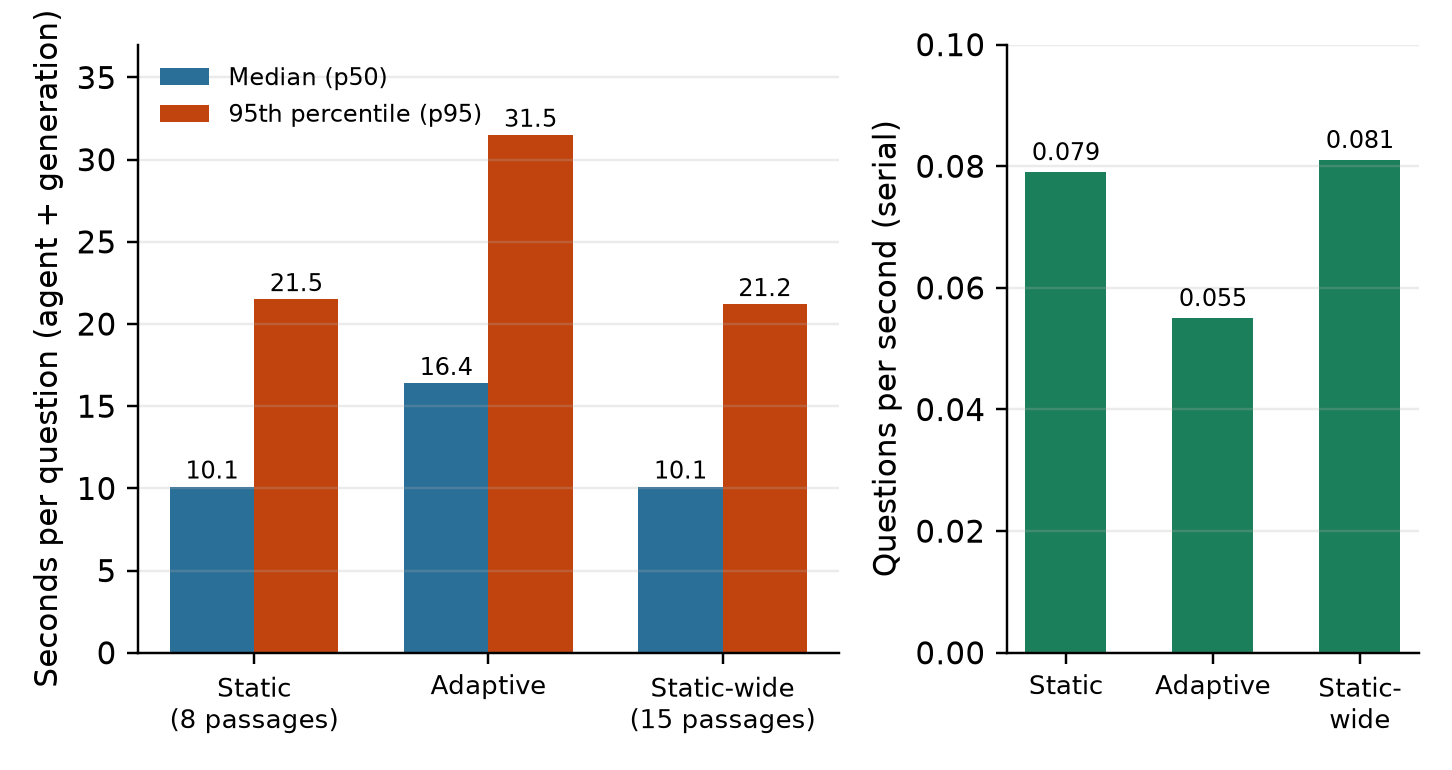
\includegraphics[width=0.92\linewidth]{images/latency-by-arm.png}
\caption{Held-out latency per question (left; agent plus generation time, one A40, serial requests) and throughput (right) by arm, the values of \hyperref[tab:perf]{Table~\ref*{tab:perf}}. The retry loop raises median latency by about 56\% and lowers throughput by about 30\%.}\label{fig:latency}
\end{figure}
Generation dominates: retrieval and fusion take 0.04\,s per question on the cluster CPU, against about 12\,s for the answer. The agent loop adds a mean 5.6\,s per question, 251 critic calls over 200 questions, and raises median latency by about 56\% (16.5 against 10.6\,s) and lowers throughput by about 30\%, for a recall gain of 0.013 (Section~\ref{sec:agent-heldout}). The critic's own token use was not recorded, so the adaptive arm's token total is a lower bound. There is no per-call monetary cost, because the model is served locally; GPU time was 2\,h 23\,min for the three arms. The RAGAS judge (Q4.5) was a paid hosted model: scoring the two arms took about 2.5 hours and cost about 0.63 Singapore dollars, as reported by the member who ran it. Concurrent throughput was not measured: calls were serial, and these figures are not a scaling benchmark.

\begin{review}{Q4.6: AI-suggested five-star implementation self-check}
\draftreview{P4}{P5, P6, P1, P2}{Following the evaluation handoff, P4 verifies final agent timing and cost; P5 checks GPU/model records; P6 verifies local UI timings and calculations; P1/P2 check historical retrieval measurements.}
\colorbox{yellow!45}{\strut\textbf{DONE FOR DRAFT --- P1}}\par
Approved by Junlin Yin on 6 November 2026 for the source attribution and wording of historical retrieval measurements. This approval does not certify a timing rerun or final GPU performance. Other owners' reviews remain pending.\par\smallskip
\colorbox{yellow!45}{\strut\textbf{DONE FOR DRAFT --- P5}}\par
Approved by Junyu Hu on 6 November 2026 for the model/GPU record and the final generation timings. P4's end-to-end benchmark and P6's local timing review remain pending.\par\smallskip
\aistars{3}\quad\textbf{Provisional AI assessment (7 November 2026, post-review): 3/5 stars.} This is an editorial assessment of the documented evidence, not a course grade or human sign-off. The report separates demonstration, historical retrieval, generation-only and end-to-end timings and supplies hardware, serial-request boundaries, percentiles, throughput, failures, generator tokens and reported judge cost. It discloses missing critic tokens and avoids a concurrency claim. Generation-only and end-to-end medians are now computed over the same 200 records with one percentile convention and agree. Startup, concurrent load and repeated-run variability are unmeasured, so the results describe observed serial performance rather than a scaling benchmark.
\end{review}


\section{Downstream innovations and ablation (Q5)}
\subsection{Bounded evidence-gap retrieval}
The agent plans evidence requirements, retrieves passages and asks a critic whether evidence is sufficient. Typed gaps such as \texttt{MISSING\_RESULT} guide a rewritten query and optional section targeting. The loop permits at most two retries, preventing unbounded search. The critic reads the generator's clipped view and must supply an evidence quote that code checks against the supplied text, allowing punctuation differences, one changed word and ellipsis elisions. This check provides traceability, not the correctness of the critic's conclusion.

\begin{table}[htbp]\centering
\caption{Agent development evidence recovery: 32 mapped-evidence questions from a 40-question slice. These results are reported in the team development record, not final QA scores.}\label{tab:agent}
\begin{tabular}{lrrr}\toprule
Arm & Mean evidence recall & Complete evidence & Mean passages\\\midrule
Static top five & 0.740 & 22/32 & 5.00\\
Adaptive top five / round & 0.771 & 23/32 & 5.95\\
Static top eight & 0.885 & 26/32 & $\leq 8$\\
Static top ten & 0.974 & 30/32 & $\leq 10$\\\bottomrule
\end{tabular}
\end{table}
The generator-view critic run (job 51172) improves mean evidence recall over static top five by 0.031, with a reported 95\% paired bootstrap interval of [0.000, 0.094] (2,000 resamples). At a matched passage budget, its difference from plain retrieval is $-0.042$, with interval [$-0.135$, 0.062]. Neither supports a reliable adaptive advantage. Static top eight recovers substantially more evidence on this slice. The agent audit further reports that 95.7\% of retries add no gold passage and 56.5\% occur when all gold is already retrieved. These observations suggest that critic calibration and stopping, rather than query wording alone, limit this implementation.

\begin{review}{Strength and provenance of agent evidence}
The development table and intervals are transcribed from the agent experiment contribution (jobs 50701, 50977, 51172, 51521; the cluster outputs are in the team's delivery archives). The held-out tables below are scored from job 51585 with the frozen record \texttt{configs/p4\_freeze.json}; the scoring script refused any run whose manifest differed from the record. Each configuration was run once. Bootstrap intervals resample questions, not papers, unlike the paired retrieval comparison above. Part of the held-out list (40 questions) was read by the agent developer before the freeze, hence the 160-question column.
\end{review}

\subsection{Held-out evaluation of the agent}\label{sec:agent-heldout}
The configuration was frozen on 6 November 2026 (code commit \texttt{ad02d51}) and run once on the 200 held-out questions: top eight per round, no reranking, at most two retries, a Qwen3-8B critic reading the generator's view, and answers from the same generator in every arm, each passage cut at 1{,}200 characters. All 200 questions are answerable and have mapped gold. Table~\ref{tab:heldout} gives mapped-evidence recall.
\begin{table}[htbp]\centering\small
\caption{Held-out mapped-evidence recall by arm (job 51585). Complete evidence in brackets.}\label{tab:heldout}
\begin{tabular}{lrrr}\toprule
 & Static, top eight & Adaptive & Static-wide (15)\\\midrule
All 200 questions: recall & 0.858 & 0.871 & 0.953\\
\quad complete evidence & 154 & 157 & 183\\
\quad mean passages & 7.97 & 8.28 & 13.95\\
160 questions not annotated by P4: recall & 0.881 & 0.897 & 0.959\\
\quad complete evidence & 127 & 130 & 148\\
\quad mean passages & 7.98 & 8.32 & 13.97\\\bottomrule
\end{tabular}
\end{table}
Paired differences (mean per-question recall, 95\% bootstrap interval, 2{,}000 resamples, seed 0): adaptive minus static top eight is $+0.013$ [0.001, 0.028] on 200 questions and $+0.016$ [0.000, 0.038] on the 160. Against plain retrieval over the same number of passages (8.28 and 8.32 on average) the matched-budget difference is $+0.001$ [$-0.014$, 0.016] and $+0.009$ [0.000, 0.025]. The loop raised recall on 4 of 200 questions (three reached complete evidence), lowered it on none, and left 196 unchanged. Reading more passages is better than retrying: plain top ten recovers 0.897 and top fifteen 0.953 (Table~\ref{tab:depth}), against 0.871 for the loop at 8.3 passages. The generator renders at most eight passages, so the fifteen-passage figure shows headroom for retrieval, not evidence the answer step used.

The loop was expensive for this gain. It ran retries on 45 of 200 questions (88 retries); 95.5\% added no gold passage, 62.5\% were made when all gold was already retrieved, and 46.6\% added no new passage. The depth-8 development check (job 51521) predicted this closely (90.5\%, 61.9\% and 40.6\%). The critic returned a model verdict for 95.8\% of its calls and fell back to the rules for 4.2\% (10 of 239). Two thirds of its ``insufficient'' verdicts (54 of 83) were issued with all gold already in view, and 29 of its 156 ``sufficient'' verdicts were issued with gold missing.

\paragraph{Abstention.}
The held-out list has no unanswerable question, so the correct-refusal rate and the proposed refusal gate cannot be assessed on it; the gate remains disabled as fixed before the run. The critic was unsatisfied after its last round on 22.0\% of the answerable questions (21.9\% on the 160), against the 5\% the gate allows. The generator refused the same six questions in every arm, and the critic's own ``insufficient information'' stop added three more in the adaptive arm; because every question is answerable, those three are false refusals (1.5\%) caused by the loop.

\paragraph{Answer quality.}
The generated answers were scored against the QASPER reference answers with the project's proposed scorer (normalized exact match and token F1, best matching reference; policy version 0, not the official QASPER evaluator). Exact match is 0.005 in every arm (one question of 200), because the generator writes sentences and the references are mostly short spans, so we rely on F1. Mean F1 is 0.368 for static top eight, 0.366 for the adaptive arm and 0.368 for the fifteen-passage arm. The paired difference, adaptive minus static, is $-0.002$ [$-0.011$, 0.006] on all 200 questions (174 papers) and $+0.0001$ [$-0.007$, 0.008] on the 160 not annotated by P4 (142 papers; 1{,}000 paper-level bootstrap resamples, seed 42). The adaptive arm answered 191 questions against 194 for static (coverage 95.5\% against 97.0\%): its three extra refusals are the critic's. Two answers per arm were downgraded after a parse error and count as failures in the scorer, which is why it reports four refusals for the static arm where the generator's own count is six. All 200 questions are answerable, so the unanswerable-correctness metric is not available. Answer-level RAG metrics from an LLM judge (Q4.5) point the same way: faithfulness is 0.892 for the static arm and 0.907 for the adaptive arm, response relevance 0.854 for both and context precision 0.578 against 0.577, and none of the paired differences (adaptive minus static, over the questions answered in both arms) has an interval that excludes zero. Faithfulness is scored only on answered questions, and the adaptive arm answers three fewer.

\paragraph{Reading.}
On unseen questions the loop behaves as it did on the development slice. It found a gold passage that plain top-eight retrieval missed on 2\% of questions, at the price of 88 retries, about 5.6\,s of agent time per question and three false refusals, and it does no better than reading the same number of passages; the answers it produces score no better (F1 0.366 against 0.368). All of this is at the primary 1{,}200-character budget; part of the loop's waste comes from the clipped view the critic reads (Section~\ref{sec:context}). The result does not support the claim that evidence-gap-driven retrieval improves recall. It supports the narrower claims that the loop never lowered recall, that its critic is usable but over-strict, and that retrieval depth is the factor that matters.

\subsection{Context budget: a post-hoc sensitivity analysis}\label{sec:context}
The generator renders at most eight passages and cuts each at a character limit. The primary result, whose configuration was fixed before any held-out question was run, used 1{,}200 characters; every result above is from that run. After the primary run had finished, we repeated the configuration with 2{,}500 characters per passage, first on the 40 development questions and then on the same 200 held-out questions. Both are \emph{post-hoc sensitivity analyses}: they were decided with the primary result known, they are not part of the frozen protocol, and they do not replace the primary result, which stands unchanged.

On the development slice (one run per cell; 32 answerable and 8 unanswerable questions; the critic and the generator read the same budget) the larger budget gives better-grounded citations and a cheaper loop (Table~\ref{tab:context}). Gold citation recall rises by 0.053 (static) and 0.043 (adaptive) and gold citation precision by 0.039 and 0.036; the adaptive arm makes 18 retries instead of 32 and detects 10 gaps instead of 18, because the critic sees more complete text. It also costs a little refusal calibration: of the 8 unanswerable questions, 5 are answered at 1{,}200 characters and 6 at 2{,}500, the extra one with a sentence that does not answer the question; answerable questions stay at 31 of 32. The loop's own gain in gold citation recall over static is $+0.032$ at 1{,}200 and $+0.022$ at 2{,}500 characters, and its gain in citation precision is about zero at both. These are one run on 40 questions without intervals, so we read them as suggestive.
\begin{table}[htbp]\centering\small
\caption{Context-budget check on the 40 development questions (post-hoc; one run per cell).}\label{tab:context}
\begin{tabular}{lrrrr}\toprule
 & Static 1{,}200 & Static 2{,}500 & Adaptive 1{,}200 & Adaptive 2{,}500\\\midrule
Answered / refused & 36 / 4 & 37 / 3 & 36 / 4 & 37 / 3\\
Gold citation recall & 0.694 & 0.747 & 0.726 & 0.769\\
Gold citation precision & 0.580 & 0.619 & 0.577 & 0.613\\
Mean rounds & 1.00 & 1.00 & 1.80 & 1.45\\
Retries & 0 & 0 & 32 & 18\\
Gaps detected & 6 & 6 & 18 & 10\\\bottomrule
\end{tabular}
\end{table}
\paragraph{Held-out sensitivity at 2{,}500 characters.}
The same 200 held-out questions were run once more at 2{,}500 characters (job 51705) and scored afterwards with the same frozen scripts. \todo{held-out result at 2{,}500 characters (job 51705) not yet scored: add one row per arm next to the primary result, labelled post-hoc}


Claude (Anthropic) was used through Claude Code to assist with implementing and testing the agent and experiment scripts, scoring the held-out run, and drafting the agent chapter and documentation; the author reviewed and ran these.

\subsection{Grounded answers and refusal}
Closed citation IDs, structured claim provenance, explicit refusal and validation make answer support inspectable. They target a practical failure: a fluent answer can contain numbers or claims that the retrieved text does not justify. However, their individual contribution to faithfulness has not been measured.

A proposed rule that would force refusal whenever the critic remains unsatisfied is disabled. In job 51172 it would refuse six of eight unanswerable questions but also nine of 32 answerable questions (28.1\%), exceeding the proposed 5\% false-refusal limit. In a separate generated-answer development run (job 51175), both static and adaptive arms refuse three of eight unanswerable questions; answer correctness has not been scored. The loop therefore has no demonstrated refusal-quality gain.

\subsection{Ablation: what was and was not isolated}
The handout asks for the contribution of each innovation alone and together. Two components were varied (query rewriting through the critic-controlled retry loop, and reranking) and Table~\ref{tab:ablation} shows what exists for each cell. Rewriting off and on are the static and adaptive arms of the held-out run. Reranking was compared with plain RRF at the retrieval level only: on the 200-question relevance pool (Table~\ref{tab:retrieval}) it lowered all four metrics, and in an earlier paired run on the development items it lowered recall at every depth (top five 0.724 against 0.740, top ten 0.885 against 0.974). No arm with reranking was run on the held-out questions, and none combines it with the loop: the freeze record fixed the arms before the run and forbids adding arms after the results are known. The answer-quality columns are therefore incomplete, and we do not claim separate answer-quality gains for rewriting, reranking or post-generation validation.
\begin{table}[htbp]\small\centering
\caption{Ablation of rewriting and reranking. Mapped-evidence recall and latency are from the held-out run (200 questions); ``not run'' marks cells that were not run.}\label{tab:ablation}
\begin{tabularx}{\linewidth}{Ycccccc}\toprule
Configuration & Rewriting & Reranking & Recall & EM/F1 & Faithfulness & p50 (s)\\\midrule
Neither (static) & Off & Off & 0.858 & 0.005 / 0.368 & \pending & 10.1\\
Rewriting only (adaptive) & On & Off & 0.871 & 0.005 / 0.366 & \pending & 16.4\\
Reranking only & Off & On & not run & not run & not run & not run\\
Both & On & On & not run & not run & not run & not run\\\bottomrule
\end{tabularx}
\end{table}
\subsection{Examples from the held-out run}
Three held-out questions illustrate what the loop does well and badly. All three are among the 160 that P4 did not annotate; they were chosen from the four questions where the loop gained evidence and the three where its critic refused, and are explanations, not an estimate of frequency. Reference answers are QASPER's.

\textbf{A gain.} ``What QA system was used in this work?'' (paper \texttt{1908.10149}; reference: the Rasa natural language understanding framework). Plain top-eight retrieval misses the one gold passage, from the section ``Question Answering System''. The static arm answers that the system is ``a baseline QA system that provides a top-10 ranking'', citing three passages that do not contain the answer. The adaptive arm retrieves again twice with the query extended by ``name baseline'' and then ``name''; the second retry retrieves the gold passage, and the answer, ``based on the Rasa natural language understanding (NLU) framework'', cites it.

\textbf{A partial gain.} ``What types of social media did they consider?'' (paper \texttt{1809.01202}; reference: Facebook status update messages). The static arm answers ``tweets and social media texts in general''. After one retry with the query extended by ``dataset experimental setup evaluation metrics'', the adaptive arm retrieves the dataset passage (``3,268 random Facebook status update messages'') and cites it, but still adds ``and tweets'' from another passage, so the answer is better supported and not fully correct.

\textbf{A failure caused by the loop.} ``What language is the data in?'' (paper \texttt{1903.11437}; reference: English, German and French). The mapped gold passage, about Europarl data ``in several languages'', is already among the eight passages of the first round. The static arm answers ``English'' (partly right, and not citing the gold passage). The critic reads the same eight passages, concludes that none states the language and stops with \texttt{INSUFFICIENT\_INFORMATION}, so the adaptive arm refuses. A critic that is over-strict turns a partly correct answer into a refusal; it did so for three of 200 questions.

\begin{review}{Q5: AI-suggested five-star implementation self-check}
\draftreview{P4}{P5, P2, P6}{P4 verifies agent experiments, matched budgets and negative findings; P5 reviews grounding/refusal and answer quality; P2 checks reranking ablations; P6 cross-checks comparisons, uncertainty and tables.}
\aistars{2}\quad\textbf{Provisional AI assessment: 2/5 stars. Target: 5/5 --- strong implementation.} This is an editorial assessment, not a course grade. The bounded agent and grounding checks are implemented, and the current negative development findings are appropriately qualified. For five stars, reviewers should complete the controlled component ablations, compare answer quality and latency at stated budgets, and supply verified cluster outputs plus a reviewed success/failure example. A well-supported negative result can meet the target; an improvement is not required. Avoid claiming separate benefits from rewriting or validation without an isolating comparison.
\end{review}


\section{Conclusions, limitations and future work}
Current evidence supports hybrid retrieval as a useful baseline and argues against retaining this reranker configuration. On the frozen held-out run, increasing the initial retrieval depth recovers more evidence than adaptive retries: the evidence-gap loop adds 0.013 to the mapped-evidence recall of static top-eight retrieval, adds nothing over reading the same number of passages, and costs about 60\% more median latency. The system provides a working route from a scientific question to a cited answer, and its answers score a token F1 of 0.368 without the loop and 0.366 with it, so the loop's extra model calls bought no measurable answer quality; an LLM judge finds the same faithfulness, relevance and context precision for both arms within its noise (Q4.5). Annotation included AI assistance, and the disagreement reviewer had labelled some disputed pairs. These limitations, the reading of 40 held-out questions by the agent developer before the freeze, the absence of unanswerable questions in the held-out list, and context clipping qualify the findings. The frozen retrieval comparison does not establish held-out downstream performance. Final evaluation should determine whether the agent's additional model calls provide an answer-quality benefit under a fixed evidence budget. A larger per-passage context budget is the most promising next step: in a post-hoc check it improved citation grounding and halved the critic's retries on the development slice (Section~\ref{sec:context}), but it has not been adopted as the primary configuration.

Future work should first address these limitations. Sentence-aware evidence selection or a larger context budget could reduce the loss of useful text through truncation; both should be tested against the current prompt budget. The critic should be calibrated to avoid unnecessary retries and evaluated against static top-eight retrieval at comparable evidence and latency budgets. Stronger evaluation could add independent third-person review of disagreement resolutions, a fresh downstream evaluation set frozen before system selection, and repeated runs to quantify variability. Finally, indexing table and figure text could extend coverage beyond the current full-text passages. These are proposed experiments; their effects on answer quality and cost remain to be measured.

\clearpage
\section{AI-use disclosure}
OpenAI Codex and Anthropic Claude Code assisted with report drafting and editing, LaTeX and diagram preparation, reference discovery, code implementation and testing, and checks of reported results against saved project outputs. Claude Code also assisted with implementing and executing the evaluation scripts for the held-out run. AI assistance with technical understanding during annotation, the earlier batch records and the separate disagreement-resolution process are described in Section~\ref{sec:annotation}. These tools were used separately from the language models evaluated within the QA system. The authors take responsibility for the submitted code, analysis, citations, results and final text.

\bibliographystyle{plainnat}
\bibliography{references}
\end{document}
